\documentclass[msc]{ppgccufmg}    % ou [msc] para disserta��es
                                  % de mestrado. Para propostas ou
                                  % projetos, usar [phd,project],
                                  % [msc,proposal], etc.

\usepackage[english]{babel}       % se o documento for em ingl�s
\usepackage[latin1]{inputenc}
\usepackage[T1]{fontenc}
\usepackage{type1ec}
\usepackage[a4paper,
  portuguese,
  bookmarks=true,
  bookmarksnumbered=true,
  linktocpage,
  colorlinks,
  citecolor=black,
  urlcolor=black,
  linkcolor=black,
  filecolor=black,
  ]{hyperref}
\usepackage[square]{natbib}

\usepackage{adjustbox}
\usepackage{array}

\newcolumntype{R}[2]{
    >{\adjustbox{angle=#1,lap=\width-(#2)}\bgroup}
    l
    <{\egroup}
}
\newcommand*\rot{\multicolumn{1}{R{45}{1em}}}

\usepackage{booktabs} % For formal tables
\usepackage[ruled]{algorithm2e} % For algorithms
\renewcommand{\algorithmcfname}{ALGORITHM}
\SetAlFnt{\small}
\SetAlCapFnt{\small}
\SetAlCapNameFnt{\small}
\SetAlCapHSkip{0pt}
\IncMargin{-\parindent}

\usepackage{graphicx}
\usepackage{mathtools}
\usepackage{amsfonts}
\usepackage{amsmath}
\usepackage{multirow}
\usepackage[cal=boondox]{mathalfa}
\usepackage{pgfplots}

\usepackage{tikz}
\usetikzlibrary{arrows,automata}

\DeclareMathOperator*{\argmax}{arg\,max\,}
\renewcommand{\arraystretch}{1.2}

\usepackage{filecontents}

\begin{document}

\ppgccufmg{
  title={Named Entity Recognition on HTML: Name Extraction from Faculty Directories},
  authorrev={de Freitas Veneroso, Jo�o Mateus},
  cutter={D1234p},
  cdu={519.6*82.10},
  university={Federal University of Minas Gerais},
  course={Computer Science},
  portuguesetitle={Reconhecimento de Entidades Nomeadas em HTML: Extra��o de Nomes de Diret�rios Acad�micos},
  portugueseuniversity={Universidade Federal de Minas Gerais},
  portuguesecourse={Ci�ncia da Computa��o},
  address={Belo Horizonte},
  date={2019-07},
  advisor={Berthier Ribeiro-Neto de Ara�jo},
  approval={pics/approvalsheet.eps},
  abstract=[brazil]{Resumo}{resumo},
  abstract={Abstract}{abstract},
  dedication={dedicatoria},
  ack={agradecimentos},
  epigraphtext={$ x = 2 $.}{Unknown},
  keywords={Reconhecimento de Entidades Nomeadas, Extra��o de Informa��o, Aprendizado de M�quina},
}

\chapter{Introduction}

The amount of data generated by almost every imaginable human endeavor is increasing at 
an accelerating pace, and the astonishing growth of the Web is perhaps the most important 
manifestation of this movement. The recurrent appearance of terms such as \textit{Big Data} 
and \textit{Artificial Intelligence} in mass media testify to the growing attention 
devoted to this topic. People, companies and academia are all interested in taming the
colossal flood of data, each for their own reasons. The Web is a practically endless 
repository of knowledge, but meaningful information gets lost over torrents of unimportant 
data, and to extract structured information from this imense haystack we need incredibly 
sophisticated solutions.

\textit{Web Information Extraction} methods are often employed when there is a need to 
extract massive amounts of structured information from webpages. Some examples of 
these needs are extracting product descriptions and their prices from online 
shops, or extracting person names and their relationships from news texts. 
HTML documents most often lie in between the structured/unstructured data paradigm. This
means that they are not structured in the same sense that a relational database is structured, 
neither are they unstructured in the same sense that plain text is unstructured. The way that
elements are organized and displayed in a webpage contribute to their meaning,
yet we cannot expect that these organizational patterns will be completely constrained 
by an underlying set of rules. Patterns tend to follow some guidelines but they are in 
no way subject to strict rules. 

Traditional \textit{Web Data Extraction} (WDE) methods often relied on the identification of
webpage patterns to build wrappers, that are simple programs aimed at extracting relevant 
entities from text by identifying their common boundaries. These programs were somewhat prone to failure 
when the webpage changed, and for this reason they demanded constant maintenance. Some improvement 
was made with the invention of automatic wrapper generators such as WIEN by \cite{Kushmerick2000}, 
Soft Mealy by \cite{Hsu1998} and STALKER by \cite{Muslea1999}, that aimed to reduce the cost
of wrapper maintenance. However, wrappers generated by these systems only worked well on 
webpages with a very similar structure (e.g. product listings from Amazon). In fact, the
problem of cross website \textit{Web Data Extraction} seems far from solved in newer 
approaches such as Knowledge Vault by~\cite{Dong2014} and AutoRM by~\cite{Shi2015}, to cite
a few.

Comparatively, statistical machine learning provides more robust and flexible methods
to \textit{Web Data Extraction}. In recent years, we saw amazing progress in 
the field of \textit{Natural Language Processing} (NLP) that is extremely relevant for
the WDE community, particularly with the introduction of \textit{Deep Neural Networks} 
for \textit{Sequence Labeling} by~\cite{Collobert2011}. But, these advancements were 
not widely incorporated by WDE systems. Also, most of the attention of the NLP community 
is devoted to solving \textit{Information Extraction} tasks in plain text, and more 
especifically news texts.
However, the difference between some types of webpages and news texts is significant, so
\textit{Information Extraction} systems trained in news datasets tend to perform very poorly 
in WDE tasks. 

A concrete example of a WDE problem that demands the type of
flexible solution provided by statistical machine learning methods is the extraction of 
researcher names from faculty directories. Automatically extracting researcher information 
from university websites is important, for example, to construct researcher affiliation databases 
and compare the academic impact of research groups using bibliographic indices as
was done by~\cite{Ribas2015a}. This particular problem can be solved with
machine learning methods of NER, as long as we take care of the specificities of HTML. 

In this dissertation, we compare different machine learning approaches to 
sequence labeling on HTML by evaluating their performance in the researcher 
name extraction task. With this purpose in mind, we introduce a novel NER dataset 
with labeled entities, consisting of faculty directories from universities across the world. 
We compare the models in terms of their Precision, Recall, F-scores and their 
overall complexity. The tested models were \textit{Hidden Markov Models} (HMM) up to third 
order, \textit{Conditional Random Fields} (CRF), and a range of \textit{Deep Learning} 
architectures based on \textit{Bidirectional Long Short-Term Memory Networks}. We also 
introduce three strategies that can boost the performance of sequence labeling methods for
HTML. The self-training strategy for HMMs, the Self-Attention layer with HTML features 
for \textit{Neural Networks}, and the direct \textit{F-score} optimization, also 
for \textit{Neural Networks}.

The usability of the evaluated models is not limited to the particular problem of researcher
name extraction. By reliably detecting named entities on HTML, we can improve the performance 
of existing WDE approaches or even construct an end-to-end architecture that
solves cross website extraction with good flexibility. Also, the researcher affiliation database
constructed with the application of these methods can be used later on bibliometric
studies.


\section{Motivation}

The practical motivation for this dissertation stems from the need to acquire reliable 
affiliation information of reseachers from many fields across the world to conduct a
bibliographic analysis of their scientific impact. Acquiring this data manually is 
impractical because of the sheer number of universities and researchers in the 
world~\footnote{The field of Computer Science alone has more than 2,200,000 researchers 
listed in https://dblp.uni-trier.de/.}, so we must resort to automatic methods. A form
of building a reliable affiliation database is to crawl university websites, find the 
faculty directories for each department, extract researcher names and link these names 
to their public profiles (when they exist). 

The crawling stage is relatively simple once we have a somewhat reliable way of 
detecting faculty webpages, but the extraction stage is trickier. Faculty listings
vary widely between different universities, and they are not always available in English,
so we need an extraction system that can handle the possible variations without having
to be trained again for each website.

There is a lack of \textit{Web Data Extraction} methods that can handle extraction
tasks across different websites. Also, \textit{Named Entity Recognition} research 
that could be useful to solve this problem seems entirely focused in detecting 
named entities in plain text. Both of these facts lead to the conclusion 
that, to peform the researcher name extraction task, we either need a new WDE method that
can handle cross-website extraction or a new labeled dataset specific for this extraction
task. 

More generally, many \textit{Information Extraction} tasks in the web share a common
factor with the researcher name extraction task. That is, they need to extract similar
entities from different webpages. An example would be comment extraction from blog
posts. Another tasks that shares a similarity with the researcher name extraction task
is \textit{Named Entity Recognition} in tweets, because of the lack of context in tweets,
NER methods trained in news corpora tend to perform badly for more or less the same reasons 
they perform badly in other HTML extraction tasks.

Finally, \textit{Information Extraction} is a very broad field, so systems that perform
well in a specific scenario are not likely to be as effective in other cases. Therefore,
when possible, it is desirable that the models be as simple as possible, so we can fine
tune them for specific extraction tasks. Taking this in consideration, we want to find 
the best \textit{NER} methods for a specific task, but trying to derive general conclusions
about their expected performance in other similar tasks.

\section{Objective}

The main objective of this dissertation is to find the best NER method for the web
in terms of its Precision, Recall, and F-scores in the researcher name extraction task,
and its overall complexity and flexibility.


\section{Contributions}

The main contributions of this dissertation are:

\begin{itemize}
\item \textbf{Contribution 1}: Labeled NER on HTML dataset. We introduce a labeled NER 
dataset specific for the task of extracting researcher names from faculty directories 
with the aim of comparing different extraction systems.

\item \textbf{Contribution 2}: Comparison of models for NER on HTML. We compare the 
performance of multiple machine learning approaches to NER on HTML.

\item \textbf{Contribution 3}: Self-training strategy for \textit{Hidden Markov Models}. 
We propose a self-training strategy to improve the performance of \textit{Hidden Markov Models} 
on HTML sequence labeling.

\item \textbf{Contribution 4}: Attention mechanism for Neural Networks on HTML. 
We propose an attention mechanism for improving the performance of \textit{Neural Networks} 
on HTML sequence labeling.

\item \textbf{Contribution 5}: F-score optimization for Neural Networks. We propose 
an optimization objective based on the F-score measure to control how much a 
\textit{Neural Network} values Recall over Precision.

\end{itemize}


\section{Dissertation Outline}

The organization of this dissertation takes the following structure:

\begin{itemize}
\item \textbf{Chapter 2: Problem Definition} defines the problem of researcher
name extraction and discusses how it relates to the broader problems of 
\textit{Web Data Extraction} and \textit{Named Entity Recognition}.

\item \textbf{Chapter 3: Researcher Name Dataset} presents the Researcher Name
Dataset that concerns the NER on HTML task of extracting research names from
faculty directories.

\item \textbf{Chapter 4: Techniques for Named Entity Recognition} describes 
\textit{Hidden Markov Models}, \textit{Conditional Random Fields} and 
\textit{Deep Neural Networks} for performing \textit{Named Entity Recognition}.

\item \textbf{Chapter 5: Sequence Labeling on HTML} describes variations and
improvements to the models described in Chapter 4 to handle sequence labeling
on HTML documents.

\item \textbf{Chapter 6: Experiments} presents the results of multiple experiments
with the models from Chapter 4 and 5 in the Researcher Name Dataset introduced in 
Chapter 3.

\item \textbf{Chapter 7: Related Work} describes the literature concerning 
\textit{Web Data Extraction} and \textit{Named Entity Recognition} that is 
related to the models explored in this dissertation.

\item \textbf{Chapter 8: Conclusion} discusses the conclusions to the research
questions that guided the experiments and proposes future work to be done in
the field.

\end{itemize}


\chapter{Problem Definition}

\textit{Web Data Extraction} (WDE) is the problem of \textit{Information Extraction} 
in web documents. WDE is a task constituted of many overlapping
problems that demand integrated and sophisticated solutions. Often, information
extraction tools that work exceptionally well on a given task perform poorly 
when given a slightly different task. Traditional methods of WDE
were mainly concerned with the extraction of entities described by a simple ontology
from web pages generated by the same source (e.g. collecting house prices and addresses 
from real estate portals). The extraction of complex entities from a plethora of sources 
presents a different class of problems. The former case could be solved by rigid tools
with hard coded rules that many times yielded close to perfect results. The latter case,
however, demands far more flexible approaches since the extraction tools are required to 
deal with a greater variety of page arrangements and also with entities that are ambiguously 
defined. In many aspects, the flexible extraction of entities from web pages is more similar 
to the tasks of \textit{Named Entity Recognition} and \textit{Relationship Extraction}
 from plain text than to the tasks that concerned the early information extraction methods.

Recent advancements in sequence models for natural language led to important 
breakthroughs in applications such as speech recognition, machine translation, 
sentence segmentation, and sequence labeling (which concerns us more directly). 
In fact, if we treat all sentences in a web page as sequences extracted from an 
underlying presentation graph (i.e. the DOM tree), the problem of information 
extraction can be solved through the consecutive application of three NLP tasks: 
sentence segmentation, named entity recognition, and relationship extraction. 
First, we need to segment the relevant grouping structures (e.g. sentences, rows in a table, 
items in a list). Then, we must identify relevant named entities (e.g. person names,
companies, locations). And finally, we have need to discover the relationships between 
those named entities (e.g. person X works in company Y). The work flow is the same
for plain text and web pages, but there are important differences chiefly related
to the structure of the data or rather the lack of structure.

In this dissertation, we investigate the best methods for sequence labeling on HTML. 
To evaluate these methods, we assess their performance on the task of researcher 
name extraction from faculty directories of universities across the world.
We will be mainly concerned with the task of \textit{Named Entity Recognition} but a brief
discussion of the challenges involved in the task of sentence segmentation for HTML 
will be provided in Chapter~\ref{cha:researcher_name_dataset}. The task of relationship extraction,
however, is not relevant to the problem of researcher name extraction and will not be
explored. 

The remainder of this chapter will describe in more depth the subject of this dissertation.
Section~\ref{sec:information_extraction} discusses the problem of information extraction.
Section~\ref{sec:named_entity_recognition} discusses the importance of NER
for WDE. Finally, Section~\ref{sec:researcher_name_extraction} describes the 
specific problem of Researcher Name Extraction.

\section{Information Extraction}
\label{sec:information_extraction}

\textit{Information Extraction} consists of mapping unstructured or poorly structured 
data to a semantically well defined structure. It "is the process of filling the fields and 
records of a database from unstructured or loosely formatted text"~\cite{McCallum2005}. 
Usually, the input consists of a corpus containing useful entities that
are scattered in the text and the information extraction system is responsible
for finding these entities and organizing them according to a rigid hierarchy such as
the one defined by the schema of a relational database. It must be stated that it is somewhat
misleading to refer to plain text as unstructured data, since prose has a loosely defined structure 
that ultimately renders it comprehensible. However, in the context of \textit{Information Extraction} 
we refer to unstructured data in contraposition to tabular data, which are in most cases 
easier to work with than plain text.

\textit{Information Extraction} is a multifaceted problem that spans communities 
of researchers in the fields of \textit{Text Mining}, \textit{Information Retrieval}, and 
\textit{Natural Language Processing}. That is:

\begin{itemize}
\item \textit{Text mining} is the search of patterns in unstructured text.
This may involve document clustering, document summarization, \textit{Information Extraction},
and other subtasks. 

\item \textit{Information Retrieval} is tipically concerned with the parsing, 
indexing and retrieval of documents. In this case \textit{Information Extraction} methods
can help giving a more precise answer to the user's information needs. 

\item \textit{Natural Language Processing}
is a field of Computer Science concerned with how computers process and understand natural 
language of which two subtasks, namely \textit{Named Entity Recognition} and 
\textit{Relationship Extraction}, are of special importance to \textit{Information Extraction}.
\end{itemize}

A popular application of \textit{Information Extraction} is the identification of 
entities such as people, organizations, or events in news sources and the determination
of their relations. For example, one could be interested in determining who is the CEO of a company
that was mentioned in the news or which politicians support a bill that is being considered
by Congress. Another interesting news-related application of \textit{Information Extraction} 
is tracking disease outbreaks through the extraction of disease names and locations 
from news sources and determining their relation to outline the geographical area affected 
by an epidemy as done by~\cite{Grishman2002}. 

The field of bio-informatics has also found important applications for 
\textit{Information Extraction}. The first BioCreAtIvE challenge dealt with the "extraction 
of gene or protein names from text, and their mapping into standardized gene identifiers 
for three model organism databases"~\cite{Hirschman2005}.
In the BioCreative/OHNLP Challenge 2018 defined in~\cite{Rastegar-Mojarad2018}, researchers 
were required to investigate methods of family history information extraction. Family
history is a critical piece of information in the decision process for diagnosis and 
treatment of diseases, however the main sources of data are unstructured electronic 
health records. The task is divided in two subtasks: 1) Entity recognition 
(family members and disease names); and 2) Relation Extraction (family members and
corresponding observations).

A scientific application for \textit{Information Extraction} methods that 
concerns this dissertation especifically is the 
extraction of information from research papers to populate citation 
databases and bibliography search engines such as Citeseer by~\cite{Lawrence1999}, 
DBLP~\footnote{http://dblp.uni-trier.de/}, 
Semantic Scholar~\footnote{https://www.semanticscholar.org}, and 
Google Scholar~\footnote{https://scholar.google.com/}.
The vast amount of scientific knowledge produced daily demands automatic
methods for extracting authors, titles, affiliations, references, venues 
and the year of publication from research papers and online resources such
as university websites, individual researcher home pages and conference
websites. This application is especially important to the evaluation and 
bibliometrics research communities, that are concerned with the measure of
academic impact and researcher productivity through the usage of quantitative
indices of academic impact such as the H-index~\cite{Hirsch2005} and 
P-score~\cite{Ribas2015a}. 

\textit{Web Data Extraction} works a little different from
\textit{Information Extraction} in plain text because HTML documents frequently
have more structure but less context than plain text. Relevant entities 
may occur inside tables, lists, or other types of visual elements that provide 
little to no contextual information that could give hints about their category.
Web pages have a two dimensional tabular structure that is usually more similar
to a spreadsheet than to text found in news corpora. For this reason, features
extracted from the DOM hierarchy such as element disposition, CSS classes, and
nesting structure can provide valuable information in identifying entities and
extracting their attributes. 

Most existing WDE methods are tailored to extract data 
from a single webpage, producing different compromises between efficacy and 
degree of human supervision. Usually, these methods work in two steps. In the 
record segmentation step, we seek to cluster visually and structurally 
similar webpage regions and identify repeating data records. In the attribute 
labeling stage, we seek to identify the correct attributes for each data record,
maybe resorting to regular expressions or simple dictionary matching strategies
depending on the task at hand. The outcome of each step can aid one 
another. The inner patterns of data records can help identifying attributes 
of other data records. Also, by properly identifying attributes, 
it becomes easier to determine boundaries and perform record segmentation 
correctly. 

Some tasks can likely be solved by a rather inflexible system that operates mainly with 
hard coded rules and simple regular expressions, especially if we only 
consider pages with a very similar template (e.g. Amazon product listings).
Traditional wrapper generators are well suited for this type of task. However, 
when we need to identify more 
complex and ambiguous entities such as researcher names in different 
contexts, we might be better off with a more 
flexible approach. The task of \textit{Named Entity Recognition} aims to identify
named entities (e.g. people, organizations, etc.) in plain text, but we will
that the sequence models that work well in plain text can also be employed succesfully 
in WDE, sometimes with a few alterations.

This section gives a brief introduction to \textit{Information Extraction}, but
there are many applications that were not discussed here. A more detailed view 
of the field is given in the survey by~\cite{Sarawagi2008}.

\section{Named Entity Recognition}
\label{sec:named_entity_recognition}

\textit{Named Entity Recognition} (NER) is a task in \textit{Natural Language Processing} that
aims to identify \textit{Named Entities} in a text. The NER 
problem definition first appeared as a subtask of 
\textit{Information Extraction} in the context of the Message Understanding 
Conference (MUC) promoted by the american Naval Ocean Systems Center. In 
MUC-3, the task defined in~\cite{Sundheim1991} involved extracting information on terrorist 
incidents (incident type, date, location, perpetrator, target, instrument,
outcome, etc.) from messages disseminated by the Foreign Broadcast
Information Service of the U.S. Government. In MUC-6, the 
"named entity" task described in~\cite{Grishman1996} was created with the goal of identifying the names of people, 
organizations, and geographic locations from articles of the Wall Street Journal.
In MUC-7, the task was expanded to handle multilingual evaluation and 
"Named Entities (NE) were defined as proper names and quantities of 
interest. Person, organization, and location names were marked as well 
as dates, times, percentages, and monetary amounts"~\cite{Chinchor1998}.
The shared-task at the Conference on Computational Natural Language Learning 
in 2003, defined in~\cite{KimSang2003}, concerned language-independent NER
and it is especially important because it established an enduring data format for
NER and it introduced a dataset of articles extracted from news sources that is
still used to evaluate the quality of NER systems.

NER is essentially a sequence labeling
task. That is, given a sequence of tokens, we want to attribute labels to each
token, classifying them into one of a limited set of predefined classes. Figure~\ref{fig:ner_example}
shows how to attribute Named Entity labels to a sentence according to the
format defined in CoNLL-2003. There are cases where a token may belong to more than one class because of
nested named entities (e.g. in "CoNLL 2003", 2003 is both part of a conference name and a date).
This complexity is of importance to some applications, as in~\cite{Katyar2018}, but it will not be discussed 
here, because nested named entities are not relevant to the problem of researcher name extraction
and most sequence models can be adapted to handle this special case.

\begin{figure}[h]
\centering{
% \input{pics/ner_example}
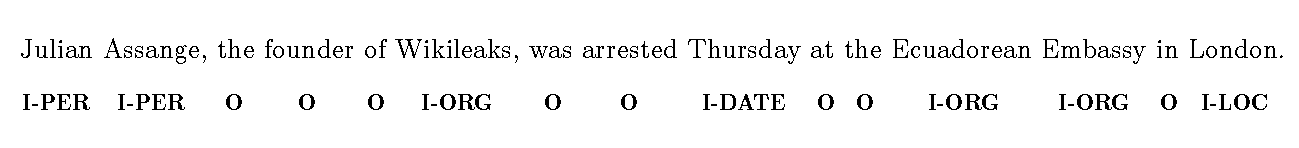
\includegraphics[width=1.0\textwidth]{pics/ner_example}
\caption{Named Entity Recognition as a sequence labeling task.}
\label{fig:ner_example}
}
\end{figure}

Regular entities such as dates and prices can be extracted with almost perfect accuracy
using regular expressions, search patterns that describe a regular language and 
that can be easily implemented in most programming languages. Entities that belong to a 
limited set, such as the names of states in a country, can also be easily extracted with
simple dictionary matching. Other types of entities, such as the ones investigated in
the CoNLL-2003 challenge, require more sophisticated methods for sequence labeling.

Some traditional statistical methods that are able to label
complex entities with decent accuracy are \textit{Hidden Markov Models} in~\cite{Leek1997}, 
\textit{Maximum Entropy Markov Models} in~\cite{McCallum2000},
and \textit{Conditional Random Fields} in~\cite{Lafferty2001}. These statistical 
approaches have had remarkable resiliency in sequence labeling tasks and still provide 
fairly good solutions because of their simplicity, speed and accuracy. However, these approaches
are rapidly being replaced by \textit{Deep Neural Networks}.

The deep learning revolution has brought great advancements to NER. Some examples are
the \textit{LSTM-CRF} by~\cite{Huang2015} and neural character representations by~\cite{Lample2016}
and~\cite{Ma2016}. Deep learning differs from classical machine learning in
regard to the levels of abstraction learned by the classifiers. Deep learning techniques combine 
feature extraction and classification in a single system. While a conventional feed-forward
neural network may perform classification by learning the weights of a single hidden layer through
backpropagation, a deep learning model is usually composed of multiple hidden layers that handle 
different levels of abstractions. In text related tasks, the first level of abstraction usually
consists of a word embedding layer, where words are mapped to a continuous vectorial space with
reduced dimensionality, and the next layer usually consists of a multi-layered 
recurrent neural network or a convolutional neural network. 

Essentially all the best scoring models to date at the CoNLL-2003 task employ some form of 
deep learning, and most often Long Short-Term Memory Networks (LSTM). When combined with pretrained
word embeddings, these models provide a powerful method for sequence labeling without
any feature engineering or dictionary matching. However, these models have 
become quite complex, constrasting with earlier approaches, that
only required the estimation of a comparatevely small number of weights. The training time
required by these deep models is many orders of magnitude larger than that of traditional approaches, 
and if we take into consideration the training of word embeddings such as Word2Vec's skip gram model 
in a billion token corpus done by~\cite{Mikolov2013}, it is no exaggeration to say that deep learning 
models increase the training time a thousandfold when compared to earlier approaches. Additionaly, 
most deep learning models require expensive hardware in the form of GPUs or 
TPUs~\footnote{Google's Tensor Processing Units "https://cloud.google.com/tpu/".}
to become practical options. 

The aforementioned sequence labeling models are exactly what we are looking for in the 
researcher name extraction task. By labeling tokens in a webpage with machine learning
models, we can extract researcher names with more flexibility than that provided by WDE 
tools.

\section{Researcher Name Extraction}
\label{sec:researcher_name_extraction}

The first objective of this dissertation is to find the best sequence models for the researcher
name extraction problem and to NER in HTML in general. 
The researcher name extraction task consists of extracting researchers names from university 
faculty listings across the world with the purpose of discovering their affiliations and linking 
their profiles to public databases such as DBLP or Google Scholar~\footnote{
  This is useful, for instance, if one needs to compare the research output of 
  departments in a country, or study international publication patterns.
}. Public researcher databases only have sparse information about author affiliation and 
even in fields for which the information is more easily available, such as Computer Science,
only a small fraction of the records have reliable affiliation information. 

\begin{figure}
  \centering
  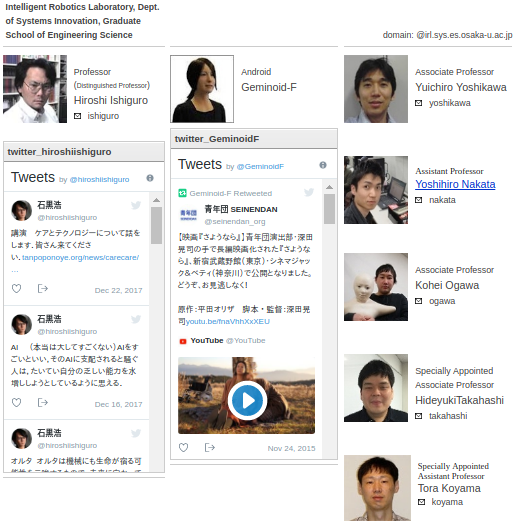
\includegraphics[width=0.75\textwidth]{pics/jap_osaka_lab}
  \caption{Example of a faculty directory}
  \label{fig:faculty_directory}
\end{figure}

To acknowledge the complexity of this task, take for example a snippet extracted from
the staff page for the intelligent robotics laboratory from Osaka University shown in 
Figure~\ref{fig:faculty_directory}. There is some structure to the way member profiles are arranged, 
but the organization is rather flexible. Other pages, even from the same website, can show very different 
patterns, ranging from tables and lists to free form.
Researcher names can appear inside plain text, similar to the case of NER in
news texts or in a more tabular structure. Names may also be part of larger sentences such as in 
"Michael Johnson Chair" and "John Doe Avenue" yielding false positives. Or they can be composed 
of common words (e.g. Summer Hall) yielding false negatives. There is no rule that fits all cases,
so we need flexible solutions.

State-of-the-art NER models trained on news datasets do not
perform well at this task, because in many webpages, textual information alone is insufficient to provide proper 
contextual information about the semantic category of a word. The absence of context demands
extraction systems to rely on information from sources outside the dataset, being them 
features extracted from unlabeled corpora obtained through unsupervised pretraining, 
dictionaries containing instances of the relevant entities, HTML structural features, 
or other clever solutions. Although, entity instances will rather 
frequently be unique occurences, rendering dictionary matching approaches
insufficient. Therefore, a key problem in the task of entity name extraction is accounting for all
possible name combinations, even those that seem unlikely. Since there is no database with all 
possible named entity combinations, we need holistic statistical methods that can handle 
unknown tokens with relative efficacy.

Considering that NER datasets built from news corpora such as CoNLL-2003 do not provide an adequate 
measure for the performance of sequence models on HTML, we introduce the NER-on-HTML dataset
to evaluate the performance of different sequence models at the researcher name extraction task
in Chapter~\ref{cha:dataset}.

Another important related task in the context of researcher name extraction is performing named 
entity disambiguation, which consists of linking the extracted named entities to a unique profile in a 
unified database. This task is called \textit{Named Entity Linking}. Roughly half the records found in 
faculty webpages can be linked to their records in public databases without great difficulty. For the 
other half, we may need to employ more complex systems or perform manual classification. This task 
is also important, but it will not be covered in the present study.

\section{Summary}

This chapter discussed the broad problem of Information Extraction in 
Section~\ref{sec:information_extraction}, presenting its challenges and relations to 
different fields of Computer Science, and showing how it encompasses the problem of 
Web Data Extraction and researcher name extraction. In 
Section~\ref{sec:named_entity_recognition} we discussed the related task of Named Entity
Recognition. Finally, in Section~\ref{sec:researcher_name_extraction} we discussed the
problem of researcher name extraction and how NER methods can be useful to solve this
task.


\chapter{NER-on-HTML Dataset}
\label{cha:dataset}

This chapter describes the dataset used to evaluate the performance of sequence models
on the WDE task of researcher name extraction. We call it the NER-on-HTML dataset.
The task consists of finding researcher names in faculty listings from university 
webpages across the world, mainly from Computer Science departments.
This would be a necessary step when linking researcher profiles from university 
websites to their entries in public databases. Unlike many
information extraction datasets, each webpage in the dataset comes from a different 
website, and therefore has a different format, what makes many information
extraction approaches impractical. The idea is to explore systems that are general 
enough to allow efficient entity extraction from different sources while requiring
no supervision between different websites. 

We collected 145 Computer Science and Engineering faculty pages from 42 different countries in
multiple languages, although the English version was preferred when it was available.
We gathered faculty webpages randomly in proportion to
the number of universities in each country\footnote{A detailed list of universities can
be found in https://univ.cc/world.php}. 

This chapter is divided as follows. Section~\ref{sec:data_description} describes the 
dataset format and how it was split in
three data files. Section~\ref{sec:evaluation} describes how the evaluation of results in this 
dataset was carried on. Section~\ref{sec:dictionary} describes how we obtained a dictionary
of relevant named entities for this dataset, and discusses some baseline results. Finally,
Section~\ref{sec:conll_comparison} compares the characteristics of the NER-on-HTML dataset
with another popular NER dataset, the CoNLL-2003 English NER dataset.


\section{Data Description} 
\label{sec:data_description}

Each of the 145 faculty pages was preprocessed and converted
to the CoNLL-2003 data format. That is, one word per line with empty lines representing
sentence boundaries. Sentence boundaries were determined by line break HTML tags
(div, p, table, li, br, etc.) in contrast to inline tags (span, em, a, td, etc.). 
Sentences that were more than fifty tokens long were also split according to the
punctuation. 
% The algorithm used for sentence segmentation is described in
% Appendix~\ref{app:html_segmenter}.

A proper HTML segmenter poses many challenges by itself. We wanted to evaluate 
models without relying on any sophisticated data record segmentation system.
In many cases, entity annotation may precede the segmentation
phase on WDE methods. Also, depending on the task (as is the case
for researcher name extraction), a good annotator that is able to work 
with raw HTML can provide a solution by itself.

Finally, all tokens were tagged using the IOB scheme put forward by~\cite{Ramshaw1999}
and used in CoNLL-2003, this is:

\begin{quote}
Words tagged with O are outside of named entities
and the I-XXX tag is used for words inside a
named entity of type XXX. Whenever two entities of
type XXX are immediately next to each other, the
first word of the second entity will be tagged B-XXX
in order to show that it starts another entity~\cite{KimSang2003}.
\end{quote}

This dataset only has entities of type person (PER), therefore a classifier has to
label each token with one of the labels: O, B-PER, or I-PER. This is an example 
sentence from the dataset:

\begin{table}[h]
  \small
  \begin{center}
    \begin{tabular}{ lllll }
      Token & Correct Label & Features \\
      \midrule
      Kasper    & I-PER & ... \\ 
      Rasmussen & I-PER & ... \\
      Associate & O     & ... \\
      Professor & O     & ... \\    
      ,         & O     & ... \\    
      Royal     & O     & ... \\    
      Society   & O     & ... \\    
      Research  & O     & ... \\    
      Fellow    & O     & ... \\    
    \end{tabular}     
  \end{center}
\end{table}

We also associated features with each token that will be discussed in
Chapter~\ref{cha:experiments}, where we consider the experimental results.

The NER-on-HTML dataset is comparable in size to other popular NER datasets.
It was divided in training, validation and test sets, which are described in 
Table~\ref{tab:dataset}. The validation set was used in the early stopping 
validation strategy to avoid overfitting classifiers, but model performance 
was only evaluated by comparing the performance in the test set, which is
never seen during training.

\begin{table}[h]
  \small
  \begin{center}
    \begin{tabular}{ lllll }
      \toprule
      Data file & Documents & Sentences & Tokens & Names \\
      \midrule
      Training    & 85  & 24728 & 110269 & 5822  \\  
      Validation  & 30  & 8743  & 36757  & 1788  \\
      Test        & 30  & 10399 & 44795  & 2708  \\
      \midrule
      Total       & 145 & 43870 & 151821 & 10318 \\
      \bottomrule
    \end{tabular}
  \end{center}
  \caption{Description of the data files in the NER-on-HTML dataset}
  \label{tab:dataset}
\end{table}


Most webpages in this dataset are faculty directories with informative
text in small passages, however long prose is not absent. 
Size and structure varies wildly, therefore some documents 
may contain up to a few hundred names whereas other documents may contain 
only twenty or thirty names. This difference in document size and characteristics 
may be problematic when comparing different extraction systems, because a system 
that performs well on some types of pages may perform poorly in other types.
To avoid this problem, we tried to keep the selection of pages as varied as possible
in the three data files.


\section{Evaluation}
\label{sec:evaluation}

The performance of classifiers in the researcher name extraction task in
the NER-on-HTML dataset was evaluated according to their Precision, Recall and F-scores
in the test set. Consider Table~\ref{tab:precision_recall}, then the Precision and Recall 
measures are defined in terms of the number of true positives, false negatives, and false 
positives made by the classifier when extracting named entities. That is:

\begin{equation*}
\text{Precision} = \frac{\text{true (+)}}{\text{true (+)} + \text{false (+)}}      
\qquad
\text{Recall} = \frac{\text{true (+)}}{\text{true (+)} + \text{false (-)}}
\end{equation*}

Precision accounts for the proportion of named entities found by the model that are 
correct relative to all predicted named entities $ m_{pos} $.
Recall is the proportion of named entities correctly predicted by the model relative to
all named entities in the dataset $ n_{pos} $. Precision measures Type I errors 
(false positives) and Recall measures Type II errors (false negatives). Partial matches are
not considered, so a classification only counts as a true positive if the entire named entity
has been correctly extracted.

\begin{table}[h]
  \small
  \begin{center}
    \begin{tabular}{ cc|cc|c }
      \toprule
        & & \multicolumn{2}{c|}{Predicted}                               & \multirow{2}{*}{Total} \\
        & & \multicolumn{1}{c}{pos} & \multicolumn{1}{c|}{neg} & \\
      \midrule
      \multirow{2}{*}{Actual} & pos & true (+)  & false (-) & $ n_{pos} $ \\  
                              & neg & false (+) & true (-)  & $ n_{neg} $ \\
      \midrule
        \multicolumn{2}{c|}{Total} & $ m_{pos} $   & $ m_{neg} $    & $ n $ \\
      \bottomrule
    \end{tabular}
  \end{center}
  \caption{Description of the data files in the NER-on-HTML dataset}
  \label{tab:precision_recall}
\end{table}

The F-score, proposed by~\cite{Rijsbergen1979}, is a composite measure that combines Precision and Recall 
with the formula:

\begin{equation}
F_{\beta} = (1 + \beta^2) \cdot \frac{\text{Precision} \cdot \text{Recall}}{(\beta^2 \cdot \text{Precision}) + \text{Recall}}
\label{eq:fscore_formula}
\end{equation}

The choice for $ \beta $ depends on the relative importance attributed to the Precision and Recall measures.
This formula "measures the effectiveness of retrieval with respect to a user who attaches 
$ \beta$ times as much importance to recall as precision"~\cite{Rijsbergen1979}. A common choice
for the value of $ \beta $ is $ 1 $, this measure is called the $ F_1 $-score. That is, we attribute 
as much importance to Recall as to Precision.

In our experiments, we considered the Precision, Recall and $ F_1 $-scores for each data file relative to 
all named entities in that file. Considering that each webpage has a different number of named entities,
this naturally privileges models that work well for pages with more named entities. 
A different approach might be to consider the averaged Precision, Recall and $ F_1 $-scores 
per webpage, privileging systems that have more regularity between different websites. However, 
this approach would cover other deficiencies, since a system that produced 100 false 
positives in a page with 500 names would account for the same level of drop in average 
Precision as a system that missed 10 names in a page with 50 names. 


\section{Dictionary}
\label{sec:dictionary}

A dictionary of named entities can be a powerful aid for sequence labeling systems,
especially when considering traditional statistical methods. For the researcher name 
extraction task, we extracted 
a list of 1,595,771 researcher names from the DBLP database and annotated tokens in the
NER-on-HTML dataset with exact and partial match tags. That is, if a sequence of tokens
corresponded exactly to a name from the DBLP list, the entire sequence was annotated as 
an exact match. Otherwise, if only some tokens in the sequence matched a name from the DBLP
list partially, the matching tokens were annotated with a partial match tag. 

\begin{table}[h]
  \small
  \begin{center}
    \begin{tabular}{ lllll }
      \toprule
      Data file & Precision & Recall & F1 & Correct names \\
      \midrule
      Training   & 0.7316 & 0.2303 & 0.3504 & 1341 of 5822 \\ 
      Validation & 0.8474 & 0.2858 & 0.4274 & 511 of 1788 \\ 
      Test       & 0.8717 & 0.3287 & 0.4773 & 890 of 2708 \\ 
      \bottomrule
    \end{tabular}
  \end{center}
  \caption{DBLP dictionary coverage in each data file of the NER-on-HTML dataset.}
  \label{tab:gazetteer}
\end{table}

To understand how this dictionary can be useful in the researcher name extraction task, 
we consider the Precision, Recall and $ F_1 $-scores for a exact dictionary matching 
strategy in each NER-on-HTML data file. The results are described in 
Table~\ref{tab:gazetteer}. These results also provide a baseline with which to compare
other methods of sequence labeling in the NER-on-HTML dataset.
This is the performance obtained by only extracting named entities that corresponded to an exact 
match. As expected, recall is very low and precision falls short of
top performing extraction methods. With this baseline in place, any useful extraction 
method should at least beat the dictionary exact matching approach.


\section{Comparison with CoNLL-2003}
\label{sec:conll_comparison}

The CoNLL-2003 dataset introduced in the \textit{Named Entity Recognition} 
shared-task in 2003 is still one of the most popular NER datasets, being used to attest 
the performance of state-of-the-art sequence labeling systems. 
The English data is composed of news stories extracted from the Reuters Corpus, and 
provides annotations for four types of entities: people (PER), organizations (ORG), 
locations (LOC), and miscellaneous (MISC), which includes entities that cannot be 
classified in one of the former groups. The statistics for the ConLL-2003 dataset 
are described in Table~\ref{tab:conll}.

\begin{table}[h]
  \small
  \begin{center}
    \begin{tabular}{ llllllll }
      \toprule
      Data file & Documents & Sentences & Tokens & LOC & MISC & ORG & PER \\
      \midrule
      Training    & 946  & 14987 & 203621 & 7140 & 3438 & 6321 & 6600 \\  
      Validation  & 216  & 3466  & 51362 & 1837 & 922 & 1341 & 1842  \\
      Test        & 231  & 3684  & 46435 & 1668 & 702 & 1661 & 1617  \\
      \midrule
      Total       & 1393 & 22137 & 301418 & 10645 & 5062 & 9323 & 10059 \\
      \bottomrule
    \end{tabular}
  \end{center}
  \caption{Description of the CoNLL-2003 English dataset}
  \label{tab:conll}
\end{table}

Considering this, it comes to mind why exactly do we need a NER dataset for HTML. 
If the CoNLL-2003 English dataset is used to both train and evaluate 
state-of-the-art models, it is to be expected that models trained in this dataset will
be able to extract the same named entities in other documents with reasonable 
effectiveness. However, this is hardly the case. By intuition, we know that tabular HTML 
documents, such as faculty listings, are very different from plain text. But now, having a
labeled dataset for NER on HTML, we can understand how different they really are.

We trained a LSTM-CRF classifier, a close to state-of-the-art sequence labeling model
introduced by~\cite{Huang2015}, using the CoNLL-2003 training set. We
relabeled the dataset, so that the classifier only extracts person entities (PER labels), and
we used the trained classifier to extract person entities from the NER-on-HTML test set.
Table~\ref{tab:conll_to_ner_on_html} describes the results obtained with this classifier
in the CoNLL-2003 test set and the NER-on-HTML test set.

\begin{table}[h]
  \small
  \begin{center}
    \begin{tabular}{ llllll }
      \toprule
      \multicolumn{3}{c}{CoNLL-2003} & \multicolumn{3}{c}{NER-on-HTML} \\
      \multicolumn{1}{c}{P} & \multicolumn{1}{c}{R} & \multicolumn{1}{c}{F1} &
      \multicolumn{1}{c}{P} & \multicolumn{1}{c}{R} & \multicolumn{1}{c}{F1} \\
      \midrule
      0.969 & 0.931 & 0.950 & 0.282 & 0.258 & 0.269 \\
      \bottomrule
    \end{tabular}
  \end{center}
  \caption{
    Performance of the LSTM-CRF model trained with the CoNLL-2003 training set and tested in
    the NER-on-HTML test set.
  }
  \label{tab:conll_to_ner_on_html}
\end{table}

The very low $ F_1 $-score obtained in the NER-on-HTML test set is even worse than our
baseline. It shows that a sequence model trained for plain text does not necessarily perform 
very well in a HTML extraction task. Also, most public NER datasets are entirely composed of 
plain text documents. 

Lets consider some differences between both datasets.
The number of documents in the NER-on-HTML dataset is much smaller: only 145 against 
1393. However, the number of sentences in the NER-on-HTML 
dataset is higher: 43870 against 22137. Also, the number of tokens in the NER-on-HTML 
is roughly half the number present in the ConLL-2003 dataset. These numbers show that 
the HTML documents relevant to the researcher name extraction task are longer than news 
stories and, more importantly, they are composed of much shorter sentences when compared 
to the text from news corpora (~3.46 words per sentence in NER-on-HTML versus ~13.62 
words per sentence in ConLL-2003). This attests to the fact that HTML provides far 
less context to be made use by sequence models. This means that the models must 
make use of information that is not present in the text.

Another aspect that differs among NER datasets is the word distributions. Word frequencies
tend to vary considerably in documents with different topics. Table~\ref{tab:frequent_words}
shows the ten most frequent words for each dataset, including punctuation signs. 
The CoNLL-2003 English dataset contains a more generic selection of terms whereas the 
subject of the NER-on-HTML becomes evident with words such as "professor" and "university" 
happening with a high frequency in the corpus. Finally, Figure~\ref{fig:word_frequency_plot}
plots the word frequencies for the hundred most frequent words in the CoNLL-2003 and 
the NER-on-HTML datasets. In both plots we have a few very frequent words and a long tail of
infrequent words. Most named entities are located in this long tail, therefore a good sequence
labeling method needs to be able to handle effectively tokens that it has seen only a couple of 
times before or even tokens that were never seen before.

\begin{table}[h]
  \small
  \begin{center}
    \begin{tabular}{ llll }
      \toprule
      \multicolumn{2}{c}{CoNLL-2003} & \multicolumn{2}{c}{NER-on-HTML} \\
      \multicolumn{1}{c}{Word} & \multicolumn{1}{c}{Frequency} &
      \multicolumn{1}{c}{Word} & \multicolumn{1}{c}{Frequency} \\
      \midrule
      the & 12310 & , & 10439      \\
      , & 10876 & - & 8140         \\
      . & 10874 & ) & 3655         \\
      of & 5502 & ( & 3641         \\
      in & 5405 & : & 3484         \\
      to & 5129 & of & 3345        \\
      a & 4731 & and & 2499        \\
      ( & 4226 & professor & 2456  \\
      ) & 4225 & university & 1611 \\
      and & 4223 & research & 1315 \\
      \bottomrule
    \end{tabular}
  \end{center}
  \caption{Ten most frequent words for the ConLL-2003 dataset and the NER-on-HTML dataset.}
  \label{tab:frequent_words}
\end{table}

\begin{figure}[h!]
  \begin{center}
    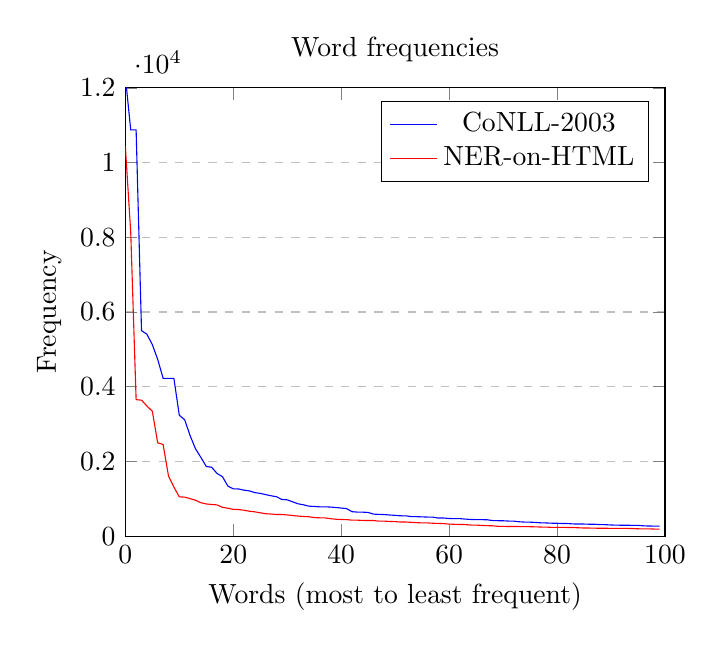
\begin{tikzpicture}
      \begin{axis}[
        title={Word frequencies},
        xmin=0, xmax=100,
        ymin=0, ymax=12000,
        ylabel={Frequency},
        xlabel={Words (most to least frequent)},
        ymajorgrids=true,
        grid style=dashed,
        legend pos=north east,
        % scaled y ticks=false,
      ]

      \addplot[color=blue, color=blue] coordinates {
        (0,12310)(1,10876)(2,10874)(3,5502)(4,5405)(5,5129)(6,4731)(7,4226)(8,4225)(9,4223)(10,3239)(11,3115)(12,2694)(13,2339)(14,2109)(15,1866)(16,1845)(17,1679)(18,1593)(19,1342)(20,1267)(21,1264)(22,1232)(23,1212)(24,1166)(25,1146)(26,1113)(27,1082)(28,1057)(29,984)(30,973)(31,920)(32,867)(33,841)(34,804)(35,796)(36,786)(37,786)(38,780)(39,768)(40,754)(41,738)(42,656)(43,645)(44,643)(45,636)(46,591)(47,584)(48,579)(49,567)(50,558)(51,546)(52,545)(53,524)(54,523)(55,517)(56,512)(57,510)(58,486)(59,486)(60,474)(61,470)(62,470)(63,457)(64,448)(65,444)(66,442)(67,441)(68,419)(69,415)(70,413)(71,405)(72,402)(73,386)(74,377)(75,375)(76,369)(77,358)(78,354)(79,348)(80,346)(81,340)(82,338)(83,328)(84,327)(85,325)(86,320)(87,319)(88,310)(89,308)(90,300)(91,296)(92,293)(93,292)(94,291)(95,289)(96,278)(97,272)(98,271)(99,271)
      };
      \addplot[color=red, color=red] coordinates {
        (0,10439)(1,8140)(2,3655)(3,3641)(4,3484)(5,3345)(6,2499)(7,2456)(8,1611)(9,1315)(10,1053)(11,1046)(12,1006)(13,963)(14,897)(15,863)(16,849)(17,838)(18,773)(19,749)(20,720)(21,713)(22,695)(23,668)(24,652)(25,626)(26,602)(27,593)(28,581)(29,580)(30,569)(31,553)(32,539)(33,527)(34,520)(35,499)(36,492)(37,490)(38,469)(39,454)(40,446)(41,444)(42,429)(43,429)(44,422)(45,420)(46,419)(47,403)(48,403)(49,394)(50,390)(51,379)(52,379)(53,371)(54,362)(55,356)(56,355)(57,346)(58,342)(59,337)(60,324)(61,318)(62,314)(63,311)(64,298)(65,297)(66,288)(67,282)(68,279)(69,265)(70,263)(71,259)(72,259)(73,258)(74,258)(75,254)(76,250)(77,245)(78,243)(79,236)(80,236)(81,235)(82,234)(83,232)(84,225)(85,219)(86,218)(87,215)(88,212)(89,212)(90,210)(91,209)(92,208)(93,208)(94,205)(95,198)(96,197)(97,196)(98,191)(99,191)
      };
      \legend{CoNLL-2003, NER-on-HTML};
       
      \end{axis}
    \end{tikzpicture}
    \caption{
      Word frequencies plot for the CoNLL-2003 dataset and the NER-on-HTML dataset.
    }
    \label{fig:word_frequency_plot}
  \end{center}
\end{figure}

\section{Summary}

In this chapter, we introduced the NER-on-HTML dataset and the researcher name extraction
task. In Section~\ref{sec:data_description} we defined the data format for the training,
validation and test data files. In Section~\ref{sec:evaluation} we discussed how to evaluate
models with the Precision, Recall and F-scores. In Section~\ref{sec:dictionary}, we 
introduced a dictionary of useful named entities for the researcher name extraction task and 
established some baseline results. Finally, in Section~\ref{sec:conll_comparison} we
compared the NER-on-HTML dataset with the popular CoNLL-2003 English dataset, showing why
a new NER dataset is necessary to complete the researcher name extraction task and why most
NER tasks in HTML will probably demand a specific dataset.


\chapter{Techniques for Named Entity Recognition}

Many tasks in Natural Language Processing, such as \textit{Part-of-Speech} tagging
and \textit{Named Entity Recognition}, can be solved by attributing labels to 
sequences of words. In NER, we want to classify words into a set of predefined
labels that determine if they are part of a named entity, but any sequence labeling 
task in NLP can be modeled generically by considering that $ X = \{x_1, x_2, ..., x_n\} $ 
is a sequence of words and $ Y = \{y_1, y_2, ..., y_n\} $ is a sequence of labels 
attributed to these words, and they are both generated by an unknown 
probability distribution. Considering that the sequence of words $ X $ is given, then
the goal of our classifier is to find: 

\begin{equation}
\label{eq:1}
Y^* = \argmax_{Y} P(Y|X)
\end{equation}

That is, the sequence of labels $ Y^* $ that maximizes the conditional probability of
$ Y $ once we have observed the sequence of words $ X $. 
Estimating $ P(Y|X) $ precisely from the relative frequencies in a labeled corpus 
is usually impractical due to the exponential increase in the number of word and label combinations that 
needs to be considered as we increase the sequence size $ n $. As $ n $ becomes large, label combinations 
will become increasingly uncommon in the dataset, what makes probability estimation less reliable. Also,
sequences that were not seen during training will always have zero probability. What is problematic, since 
most word sequences that we care about will belong to this category.
Ultimately, the difference between statistical sequence labelling models lies in the assumptions 
that we make about the distribution $ P(Y|X) $. And most statistical models of natural language make 
some very simplistic assumptions about the language structure. For example, a common assumption that is 
shared to some extent by all the models discussed in this chapter is the Markov Assumption, that will be 
discussed thoroughly in Section~\ref{sec:hmm}. Stated simply, it assumes that by looking at a limited 
history at any position in the sequence, for example the two previous words, we have sufficient information to make accurate 
predictions about the current word's label. In the related task of language modelling, that consists of predicting the next 
word in a sequence by looking at it's history, the model that looks at the two previous words to predict 
the next word is called a bigram model and the model that looks at the three previous words is called a 
trigram model.

\begin{quote}
For anyone from a linguistics background, the idea that we would choose to use a model of language structure
which predicts the next word simply by examining the previous two words - with no reference to the 
structure of the sentence - seems almost preposterous. But, actually, the lexical co-occurrence, semantic, and
basic syntactic relationships that appear in this very local context are a good predictor of the next word, and
such systems work surprisingly well. Indeed, it is difficult to beat a trigram model on the purely linear task
of predicting the next word.~\cite{Manning1999}.
\end{quote}

In other words, we do not usually evaluate the quality of statistical natural language models by how reasonable
their assumptions are, but by how instrumentally effective the models are when solving objective tasks. The 
epistemological implications of this view are manyfold, but in this work we will consider it to be valid.

In this chapter, we discuss several machine learning methods for NER. In Section~\ref{sec:hmm}, we discuss Hidden Markov 
Models, in Section~\ref{sec:crf} we discuss Conditional Random Fields, and in Section~\ref{sec:neural_networks} we 
discuss Neural Networks.


\section{Hidden Markov Models}
\label{sec:hmm}

The \textit{Hidden Markov Model} (HMM) is an expanded \textit{Markov Chain} where the sequence of observed states
depends on an underlying sequence of hidden states. A \textit{Markov Chain} is a stochastic 
model for describing sequences when the described sequences have the \textit{Markov Property}. That is, 
consider a sequence $ Y = \{y_1, y_2, \ldots, y_n\} $ in which each observed
state $ y_i, \forall i \in [1, n] $ takes its value from a restricted set of possible states
$ L = \{l_1, l_2, \ldots, l_m \} $. Sequence $ Y $ only satisfies the \textit{Markov Property} if:

\begin{equation}
P(y_i|y_{i-1}, y_{i-2}, \ldots, y_1) = P(y_i|y_{i-1}, y_{i-2}, \ldots, y_{i-k})
\end{equation}

The probability of observing state $ y_i $ at time $ i $ depends only on the $ k $ previous observed states.
When $ k = 1, k = 2, \ldots $ the \textit{Markov Chain} is said to be of first order, second order, and so on.
What the \textit{Markov Assumption} means is that, at any time, the entire history of observed states
is encoded in a limited number of previous states. So, by knowing a limited number of 
previous states, we can make as accurate predictions about the future as we would make by 
knowing all the history. Conditioned on this limited set of previous states, the future and past states 
are independent. 

A \textit{Markov Chain} can represent a wide range of phenomena such as daily temperatures in a region, 
closing prices of a stock in the financial market, yearly demographic growth, or words in a text. 
In all these cases it is a simplification of reality that makes sequences mathematically 
treatable. The extent to which this simplification will hurt our predictions depends on the 
nature of the studied phenomena. 

To see why the \textit{Markov Assumption} may introduce a problem on text related tasks, consider the following
labeled sentence: 

\begin{quote}
"[Jon Snow]$_{PER}$ is [Ned]$_{PER}$ 's son. Snow is piling up on [Winterfell]$_{LOC}$, but [Snow]$_{PER}$ is not bothered"
\end{quote}

To understand that the last mention of "Snow" refers to the person mentioned in the beginning of the sentence, we
need to keep track of distant relationships in the text that would not be captured by a \textit{Markov Model} of second 
or third order. We could consider
employing a \textit{Markov Model} of higher order to overcome this limitation, however,
considering more than three or four states at any time makes parameter estimation unreliable,
because each combination of states becomes increasingly uncommon in the training set. Also, 
when the considered number of states increases, the cost for predicting the optimal sequence 
of states quickly becomes prohibitively high. 
There are some \textit{Markov Chain} variations that try to address this problem, 
as well as the other models presented later in this chapter.
Nevertheless, in \textit{Named Entity Recognition}, HMMs up to third-order work
remarkably well despite this limitation if we add independent features to make up for the lack of a 
longer context. 

From now on, we consider all Markov Chains to be of first order (i.e. $ k = 1 $), omitting the parameter $ k $
to simplify the notation. This is not a problem since we can convert a Markov Chain of second 
order with two states $ \{A,B\}$ into a Markov Chain of first order with four 
states $ \{ AA, AB, BA, BB \} $.

We have yet not made any restrictions on the form taken by the transition probabilities 
$ P(y_i=l_b|y_{i-1}=l_a) $ besides the \textit{Markov Assumption}. But it is usual to consider 
these probabilities to be time invariant.

\begin{equation}
P(y_{i+1} = l_b |y_{i} = l_a) = P(y_i = l_b |y_{i-1} = l_a)
\end{equation}

That is, given states $ l_a $ and $ l_b $, the probability of going from $ l_a $ 
to $ l_b $ on timestep $ i $ is the same as in any other timestep. 
With this, we can calculate the probability of observing sequence
$ Y = \{ y_1, y_2, ..., y_n \} $ with:

\begin{equation}
P(Y) = \prod_{t=1}^{n} P(y_t|y_{t-1}) \\
\end{equation}

With the \textit{Time Invariance Assumption}, all parameters in our model can be described 
by a $ m \times m $ transition matrix $ \theta $ where each element $ \theta_{a, b} $ with
row $ a $ and column $ b $ holds the probability of going from state $ l_a $ to $ l_b $.
Naturally, the probabilities of row $ \theta_{a, *} $ must sum up to one since they represent
the entire scope of transition possibilities starting from state $ l_a $. For example,
consider the finite state-machine in Figure~\ref{fig:markov_graph} that describes 
a \textit{Time Invariant Markov Chain} with only two states (Name, Word), that models a sequence 
of words that can be either names or common words. The edges in this graph represent the transition
probabilities between states and the transition matrix for this Markov Chain takes the form:

\begin{equation*}
\theta = 
\begin{bmatrix}
    0.3 & 0.7 \\
    0.4 & 0.6 \\
\end{bmatrix}
\end{equation*}

\begin{figure}
\centering
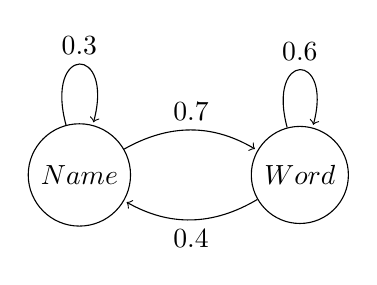
\begin{tikzpicture}[->,shorten >=1pt,auto,node distance=2.8cm]
  \tikzstyle{every state}=[]

  \node[state] (A)              {$ Name $};
  \node[state] (B) [right of=A] {$ Word $};

  \path (A) edge [loop above] node {0.3} (A)
            edge [bend left]  node {0.7} (B)
        (B) edge [bend left]  node {0.4} (A)
            edge [loop above] node {0.6} (B);
\end{tikzpicture}
\caption{Finite state machien for a Markov Chain.}
\label{fig:markov_graph}
\end{figure}

If we know the transition matrix $ \theta$ for a \textit{Markov Chain}, we can easily calculate 
the probabilities of being in each state at time $ t $. If $ \rho_t $ is a vector of 
size $ m $ with the probabilities for each state at time $ t $. Then:

\begin{equation}
\rho_{t} = \rho_0 \cdot \theta^t
\end{equation}

Where $ \rho_0 $ is the vector of starting probabilities for each state. We assume that we 
have no knowledge about the initial conditions of our \textit{Markov Chain}, so we simply 
attribute the same probability to every state at time $ t=0 $. For the remainder of the explanation,
consider that $ P(y_1|y_0) $ is the probability of $ y_1 $ given the initial vector of uniform state
probabilities $ \rho_0 $. 

Now we know how to calculate the state probabilities for a Markov Chain at any timestep, but
we still need to solve the problem of obtaining the transition matrix $ \theta $. The usual
choice is to obtain $ \theta $ such that it maximizes the probability of our labeled dataset 
with Maximum Likelihood Estimation. The likelihood of our model is given by:

\begin{equation}
\mathcal{L}(\theta; Y) = \prod_{t=1}^{n} \theta_{y_t, y_{t-1}}
\end{equation}

By defining $ \eta_{a,b} $ to be the count of transitions from $ a $ to $ b $ in $ Y $. We can write the likelihood as:

\begin{equation}
\mathcal{L}(\theta; Y) = \prod_{a, b} \theta_{a, b}^{\eta_{a, b}}
\label{eq:hmm_likelihood}
\end{equation}

Where the product is calculated over all possible transitions from $ a $ to $ b $.
The logarithm function is monotone increasing, so we can maximize the log-likelihood instead
of the likelihood for ease of calculation. With the log-likelihood, the product over transition 
probabilities becomes a sum of logarithms. The log-likelihood is defined by:

\begin{equation}
\mathcal{l}(\theta; Y) = \sum_{a, b} \eta_{a, b} \cdot log(\theta_{a, b})
\end{equation}

Then, the maximum likelihood estimator becomes:

\begin{align}
\hat\theta = \argmax_{\theta} \mathcal{l}(\theta; Y)
\end{align}

However, if we try to optimize this function as it is, we will find that
$ \hat\theta_{a, b} = \infty, \forall a, b \in [1, m] $. This happens because we did not
take into account the degrees of freedom of our model. Every row in the transition matrix must sum up to one,
so the parameters for the last row are defined by the preceding roles and the degrees of freedom 
for the model are actually $ m(m-1) $ and not $ m^2 $ as we considered before. That is, we have a
set of constraints:

\begin{equation}
\sum_{b} \theta_{a, b} = 1, \forall a \in [1, m]
\end{equation}

With the aid of Lagrange Multipliers, we can incorporate this set of constraints into our optimization 
objective and optimize the Lagrangian:

\begin{equation}
\Lambda(\theta, \lambda) = \mathcal{l}(\theta; Y) - \sum_{a} \lambda_{a} \cdot \left( \sum_{b} \theta_{a, b} - 1 \right)
\end{equation}

Setting $ \frac{\partial \Lambda(\theta, \lambda)}{\partial \lambda_a} = 0 $ simply yields the initial set 
of constraints, but by setting the partial derivatives $ \frac{\partial \Lambda(\theta, \lambda)}{\partial \theta_{a, b}} = 0 $,
we get:

\begin{eqnarray}
\frac{\partial \Lambda(\theta, \lambda)}{\partial \theta_{a, b}} & = & \frac{\eta_{a, b}}{\theta_{a, b}} - \lambda_a = 0 \\
\theta_{a, b} & = & \frac{\eta_{a, b}}{\lambda_a}
\end{eqnarray}

Finally, using the initial constraint equations, we find that:

\begin{align}
\sum_b \frac{\eta_{a, b}}{\lambda_a}  =  1 \\
\lambda_a                             =  \sum_b \eta_{a, b} \\
\hat{\theta}_{a, b}                         =  \frac{\eta_{a, b}}{\sum_{b'} \eta_{a, b'}}
\label{eq:theta_estimate}
\end{align}

Yielding a closed form expression for the maximum likelihood transition matrix. What is really convenient, 
since this is the average number of transitions from state $ a $ to state
$ b $ in sequence $ Y $. A value that can be easily calculated with our labeled dataset.

So far, we have assumed that all states $ Y $ are observable, but in \textit{NER}, only the words 
are observed, while the Named Entity labels associated with these words are not. That is why we need
another layer of complexity. The \textit{Hidden Markov Model (HMM)} differs from the \textit{Markov Chain} in that it 
does not observe the states $ Y $ directly, but rather a probabilistic function of these states. 

With the \textit{Hidden Markov Model}, we want to predict a sequence of labels $ Y = \{y_1, y_2, ..., y_n\} $ 
(i.e. the \textit{Markov Chain}) from a sequence of observed states $ X = \{x_1, x_2, ..., x_n\} $
(i.e. the words in a text, or a feature vectors with independent features). So we make an additional assumption:

\begin{equation}
P(x_i|y_{i-1}x_{i-1}, ..., y_1x_1) = P(x_i|y_i)
\end{equation}

That is, the probability of observing word $ x_i $ depends only on the current label
$ y_i $, the hidden state (e.g. PER, LOC, ORG, etc.). By making this assumption, we are
stating that if we know a token's assigned label, then we can reliably predict what are the 
probabilities that this token takes any value from a limited vocabulary. This assumption
is very problematic when we want to incorporate features other than the current word to predict
labels, because it has to assume feature independence. For this reason, other models (such as Conditional 
Random Fields) try to overcome this issue by making different assumptions, but they lose the 
closed-form expression for the Maximum Likelihood Estimator, having to resort to numerical optimization
methods.

To model the emission probability distributions $ P(x_i|y_i) $, we assume again that 
the probabilities are time invariant and that $ x_i $ takes its value from a fixed vocabulary 
with size $ V $. Similar to the transition matrix $ \theta $, we introduce a $ V \times K $ 
emission matrix $ \mu $ where each cell $ \mu_{a,b} $ represents the probability that, 
given label $ a $, we will observe the word $ b $. For example, consider the
finite state-machine in Figure~\ref{fig:hidden_markov_graph} that extends our previous 
example and defines a Hidden Markov model with two states (Name, Word), and a vocabulary of 
two words (John, Hall). The edges between the hidden states and the words represent the emission probabilities,
and the emission matrix for this HMM takes the form:

\begin{equation*}
\mu = 
\begin{bmatrix}
    0.9 & 0.1 \\
    0.8 & 0.2 \\
\end{bmatrix}
\end{equation*}


\begin{figure}
\centering
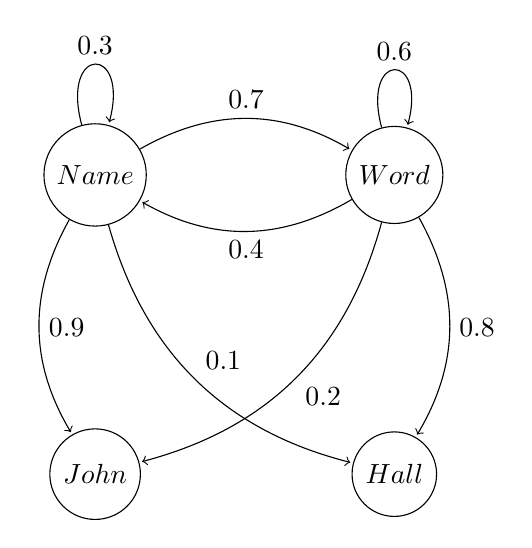
\begin{tikzpicture}[->,shorten >=1pt,auto,node distance=3.8cm]
  \tikzstyle{every state}=[]

  \node[state] (A)              {$ Name $};
  \node[state] (B) [right of=A] {$ Word $};
  \node[state] (C) [below of=A] {$ John $};
  \node[state] (D) [below of=B] {$ Hall $};

  \path (A) edge [loop above] node {0.3} (A)
            edge [bend left]  node {0.7} (B)
            edge [bend right] node {0.9} (C)
            edge [bend right] node {0.1} (D)
        (B) edge [bend left]  node {0.4} (A)
            edge [loop above] node {0.6} (B)
            edge [bend left] node {0.2} (C)
            edge [bend left] node {0.8} (D);
\end{tikzpicture}
\caption{Finite state machine for a Hidden Markov Model.}
\label{fig:hidden_markov_graph}
\end{figure}

Now, the probability of observing a vector of labels $ Y $ given a sequence of 
words $ X $ can be calculated with Bayes' theorem:

\begin{equation}
P(Y|X) = \frac{P(X|Y) P(Y)}{P(X)}
\end{equation}

Since $ P(X) $ is invariant for every sequence of labels $ Y $, we can simply 
optimize in terms of the joint probability:

\begin{equation}
P(Y|X) \propto P(X|Y) P(Y) = P(X, Y)
\end{equation}

And the log-likelihood takes the form:

\begin{equation}
\mathcal{l}(Y|X; \theta) \propto 
\sum_{a \in L, b \in L} {\eta_{a, b}} \cdot log(\theta_{a, b}) +
\sum_{c \in L, d \in V} \eta'_{c, d} \cdot log(\mu_{c, d})
\end{equation}

Where $ \eta'_{c, d} $ is a function that counts the number of emissions from state $ c $
to word $ d $. The matrices $ \theta $ and $ \mu $ are independent, so we can optimize for
the transition and emission matrices separately, therefore the procedure to find $ \hat\theta $ 
is exactly the same that we described in Equation~\ref{eq:theta_estimate}. Also, notice that
if we do the same procedure with Lagrangian Multipliers that we employed to find the MLE 
for Markov Chains, but this time we take the partial derivatives relative to 
$ \mu_{c,d} $ and set the constraints such that each line in the emission matrix must sum up
to one, we will find that:

\begin{equation}
\hat{\mu}_{c, d} = \frac{\eta'_{c, d}}{\sum_{d'}\eta'_{c, d'}}
\label{eq:mle_words}
\end{equation}

This is the expected number of times that we observe word $ d $ when we were at the hidden state $ c $. 
A closed form expression that is easy to calculate from the training data. With that, we conclude 
the maximum likelihood parameter estimation for the \textit{Hidden Markov Model}. This procedure is
only usable when we have access to labeled data, since we need to observe the correct labels $ Y $ 
to estimate $ \hat\theta $ and $ \hat\mu $. If we only have unlabeled data or partially labeled data, 
we can do the parameter estimation with the Baum-Welch Algorithm by~\cite{Baum1970}, though the results for 
NER become much less reliable.


\subsection{Smoothing}

The problem with the Maximum Likelihood Estimate derived above is that the emission probability for 
words that were not observed in the training set will always be zero. Considering that we only have a 
small dataset and even if it were much bigger we would still observe many unique words when running predictions
for unseen data, this problem needs to be addressed. By taking the Maximum a Posteriori estimate with 
uniform priors instead of the Maximum Likelihood estimate for $ \theta $ and $ \mu $, we get the Laplace
smoothed estimates:

\begin{align}
\hat{\theta}_{a, b}    =  \frac{\eta_{a, b} + 1}{\sum_{b'} \eta_{a, b'} + |L|} \\
\hat{\mu}_{c, d} = \frac{\eta'_{c, d} + 1}{\sum_{d'}\eta'_{c, d'} + |V|}
\end{align}

Where $ |L| $ is the number of labels and $ |V| $ is the size of the vocabulary.
If we consider other prior distributions for the parameters, we get different smoothed probabilities, 
but this already properly ensures that unobserved words will not receive a zero probability. The main
shortcoming with Laplace Smoothing is that it gives too much probability mass to unseen words relative
to other smoothing methods, but it performs well in practice.


\subsection{Predicting sequences}

The last task that needs to be done is to calculate the most likely sequence of labels given a sequence of
observations. To obtain this sequence, we can employ the Viterbi algorithm by~\cite{Forney1973}, which is a dynamic 
programming algorithm that calculates the probabilities for sequences with the Markov property exactly and efficiently.
As we increase the order of our HMM, this computation becomes exponentially more expensive,
but we found experimentally that for HMMs up to third order, the Viterbi algorithm is still viable. For larger windows,
a beam-search strategy can be used. For decoding the labels for CRFs and Neural Networks we also use the
Viterbi algorithm.


\subsection{Conclusion}

HMM based taggers have been successfully applied in many NLP and WDE tasks such as in the works by
\cite{Rabiner1990}, \cite{Leek1997} and \cite{Freitag2000}. The closed-form parameter estimation
makes them incredibly fast to train, also their parameters are very interpretable, making them a good 
choice for a first approximation to NER. However, these models are very simple and highly dependent on 
the right selection of features, what may outweigh the benefit of a small training cost.


\section{Conditional Random Fields}
\label{sec:crf}

With Hidden Markov Models, we tried to model the joint probability between 
words and labels $ P(X, Y) $ and derive the conditional probability $ P(Y|X) $
with Bayes Theorem. However, this is a waste of modelling effort,
since we need to assume the shape of the prior distribution $ P(X) $, but we 
only really care about the conditional problem. Thus, modelling $ P(Y|X) $ 
instead of the joint distribution would presumably be a more direct and simple 
approach. Also, to assure that the computation of $ P(X, Y) $ was feasible, we 
needed to assume feature independence, what inhibits the use of overlapping 
features that could potentially be useful in addition to words. Maximum Entropy
models for sequence labeling were created to address these issues and, among 
them, \textit{Linear Chain Conditional Random Fields} (CRF) stand out 
as the discriminative analogue to HMMs. CRFs estimate the conditional probability 
while HMMs, being generative models, estimate the joint probability.

The concept of Information Entropy established by~\cite{Shannon1948}
quantifies the amount of information expressed in a statistical distribution. 
The entropy $ H $ of a random variable Z with a probability mass function 
$ P $ is given by:

\begin{equation}
H(Z) = \sum_{z \in Z} P(z) \cdot log \left( \frac{1}{P(z)} \right)
\end{equation}

The logarithm in the entropy function can be taken in any base. The change 
of base will only provide a linear scaling of the same entropy function. When using base two,
$ H(Z) $ is essentially the expected number of bits necessary to encode the value of a
random outcome drawn from $ Z $, that is $ E \left[log \left( \frac{1}{P(Z)} \right) \right] $.
The more bits we need to use to encode the possible outcomes of a probability mass function, 
the more uncertain we are about the underlying distribution. For example, if an event has
only one possible outcome, we always know the value of a random sample, therefore
$ H(Z) = 0 $ and the entropy is minimum. On the other end, if the probability distribution is
uniform, all outcomes have the same probability, and therefore we are as uncertain as we can be
and the entropy is maximum.

The principle of maximum entropy set forward by~\cite{Jaynes1957} states that, when we do not know exactly what probability 
distribution generated a sample, the best estimate for the parameters of this probability
distribution is the one that makes the least assumptions, or the one with maximum entropy. 
This is the distribution that is closest to the uniform distribution. 
A similar argument can be made to limit the number of free parameters in the model. That is,
when comparing two models with similar predictive power, the one with the least degrees of 
freedom should be preferred. 

The principle of maximum entropy is similar to a principle in the philosophy of science called Occam's Razor, 
that states that, when there are two explanations for an outcome, the one that makes
the least number of assumptions is the best. Which is a good rule of thumb for science in general,
eventhough, ultimately, nothing guarantees that simpler models will be better.

The task of labeling word sequences can be thought of as a classification task where 
each label $ Y $ is predicted according to its context $ X $. The context is defined as 
a vector of observations that expresses useful pieces of evidence such as: the last word 
is an honorific, the current word is capitalized, the current word is "that", etc. And we
define $ k $ binary feature functions $ f_i \; \forall i \in [1, k] $ such that:

\begin{equation}
  f_i(x, y) = \begin{cases} 
    1 \text{ if } y = L \text{ and the feature is present in } x \\ 
    0 \text{ otherwise}
  \end{cases}
\end{equation}

So, at any position in the sequence, the truth statement of the feature functions can be
determined in terms of the predicted label $ y $ and the context $ x $. But, different from
HMMs, we do not assume that features are independent. Now, the \textit{Maximum Entropy} framework 
provides a compelling way for estimating the probability of a label given its linguistic context, 
that is $ P(Y|X) $. In the sequence labeling problem, we actually want to maximize the conditional 
entropy:

\begin{equation}
H(Y|X) = - \sum_{x \in X, y \in Y} P(x, y) \cdot log \left( P(y|x) \right)
\end{equation}

But, it is usual to approximate $ P(x, y) $ with $ P(y|x)\tilde{P}(x) $, because
the model prior $ P(x) $ is hard to normalize since the probability space of observations is
usually too big, while the empirical prior $ \tilde{P}(x) $ is easy to obtain.
However, if we maximize $ H(Y|X)$ subject to no restrictions, we will find that the 
\textit{Maximum Entropy} estimator will yield an uniform distribution, meaning that we are 
no better than simply predicting labels at random. So, it becomes necessary to establish 
some constraints for the optimization problem. 

The choice is more or less arbitrary, but under the \textit{Maximum Entropy} 
framework, there is a strong motivation for setting the constraints in a way that makes
the \textit{Maximum Entropy} estimator equivalent to the \textit{Maximum Likelihood} estimator
for our model. By doing it, we can make sure that the model fits the data as tightly as possible
(Maximum Likelihood), while making as few assumptions as it needs to (Maximum Entropy). 
We can get this estimator by setting the constraints such that, given the $ k $ binary feature 
functions that we determined earlier, there are also $ k $ constraints such that:

\begin{equation}
E_{P}[f_i] = E_{\tilde{P}}[f_i] \;\;\; \forall \; i \in [1, k]
\label{eq:maxent_constraints}
\end{equation}

Where $ E_{P}[f_i] $ is the model expectation of $ f_i $ and $ E_{\tilde{P}}[f_i] $ is the 
empirical expectation of $ f_i $. Or more clearly:

\begin{align*}
E_{P}[f_i]         = \sum_{x \in X, y \in Y} \tilde{P}(x)P(y|x) f_i(x, y) \\
E_{\tilde{P}}[f_i] = \sum_{x \in X, y \in Y} \tilde{P}(x, y) f_i(x, y)
\end{align*}

Additionally, we need to make sure that the probabilities sum up to one, so:

\begin{equation}
\sum_{y} P(y|x) = 1 \;\;\; \forall \; x \in X
\label{eq:maxent_constraints}
\end{equation}

We can optimize the conditional entropy subject to these constraints with Lagrangian 
Multipliers by defining the Lagrangian:

\begin{equation}
\Lambda(P, \lambda, \beta) = H(Y|X) + \sum_{i=1}^k \lambda_i (E_{P}[f_i] - E_{\tilde{P}}[f_i]) 
+ \sum_{x \in X} \beta_x \left( \sum_{y \in Y} P(y|x) - 1 \right)
\end{equation}

And solving the unconstrained optimization problem to obtain the maximum entropy 
distribution:

\begin{equation}
P^{*} = \argmax_P \Lambda(P, \lambda, \beta)
\end{equation}

The derivatives relative to $ \lambda_i $ and $ \beta_x $ yield the initial constraints, but
setting the derivative of $ P(y|x) $ to zero, we get:

\begin{eqnarray}
\frac{\partial \Lambda}{\partial P(y|x)} = -\tilde{P}(X) -\tilde{P}(X) \cdot log \; P(y|x) + \beta_x + \tilde{P}(X) \sum_{i=1}^k \lambda_i f_i(x, y) = 0 \\
P(y|x) = exp \left( \frac{\beta_x}{\tilde{P}(x)} - 1 \right) \cdot exp \left( \sum_{i=1}^n \lambda_i f_i(x, y) \right)
\label{eq:logistic_1}
\end{eqnarray}

By replacing $ P(y|x) $ in our initial probability constraints defined in Equation~\ref{eq:maxent_constraints},
we get:

\begin{eqnarray}
\sum_y exp \left( \frac{\beta_x}{\tilde{P}(x)} - 1 \right) \cdot exp \left( \sum_{i=1}^n \lambda_i f_i(x, y) \right) = 1 \\
exp \left( \frac{\beta_x}{\tilde{P}(x)} - 1 \right) = \frac{1}{\sum_y exp \left( \sum_{i=1}^n \lambda_i f_i(x, y) \right)} \\
Z(x) \equiv \sum_y exp \left( \sum_{i=1}^n \lambda_i f_i(x, y) \right)
\end{eqnarray}

By replacing $ Z(x) $ in Equation~\ref{eq:logistic_1} we finally get:

\begin{equation}
P(y|x) = \frac{1}{Z(x)} \cdot exp \left( \sum_{i}^n \lambda_i f_i(x, y) \right)
\label{eq:logistic_1}
\end{equation}

This defines a family of exponential functions with parameters $ \lambda $. To obtain the parameters
that maximize the entropy of our model subject to the initial set of constraints, we can replace this
definition back in the Lagrangian and optimize in terms of $ \lambda $. This yields the following
optimization problem:

\begin{equation}
\Lambda(\lambda) = \sum_{i=1}^k \lambda_i E[f_i(x, y)] - \sum_{x} \tilde{P}(x) \cdot log \; Z(x) 
\end{equation}

Which is identical to the log-likelihood:

\begin{equation}
\mathcal{l}(P) = \sum_{x, y} \tilde{P}(x, y) \cdot log \; P(y|x) 
\end{equation}

With this, we conclude that a model with the parametric form defined in Equation~\ref{eq:logistic_1} 
has identical maximum likelihood and maximum entropy estimators. Also, it can be proven that this 
model is unique and its optimization function is concave~\cite{Brown1986}. The classifier based on this
model is known as a logistic classifier or maximum entropy classifier. There is no closed-form expression
for finding the optimal set of parameters, but we can obtain this optimal set with numerical optimization
methods such as Stochastic Gradient Descent. Normally, this is achieved by minimizing the cross-entropy
for the exponential model, which is identical to maximizing the likelihood.

For the particular case of sequence labeling, the simplest conceivable classifier inside the Maximum Entropy
Framework would be a multinomial logistic regression that decodes each label independently. That is, given
a context $ x $, the classifier would predict a label $ y $ without taking in consideration any of the
previous or forward labels. This would be the discriminative analogue to the Naive Bayes model. However, 
the independence assumption is too restrictive for most language related tasks. 

Linear Chain Conditional Random Fields relax this assumption by jointly decoding the entire 
sequence of labels. That is, it normalizes the probabilities for the entire
sequence of labels and the feature functions also take the previous label in consideration. 
The CRF equation is very similar to the generic maximum entropy equation derived earlier. The only difference being
the assumptions about the feature functions and the joint decoding of label sequences. 
For a sequence of contexts $ X $ and labels $ Y $ with size $ n $ and $ k $ feature functions, the 
linear chain conditional random field is defined by:

\begin{eqnarray}
P(Y|X) = \frac{1}{Z(x)} \prod_{t=1}^{n} exp \left( \sum_{k=1}^{k} \theta_k f_k(y_{t-1}, y_t, X) \right) \\
Z(x) = \sum_{Y'} \prod_{t=1}^{n} exp \left( \sum_{i=1}^{k} \theta_k f_k(y_{t-1}, y_t, X) \right)
\end{eqnarray}

Where $ Y' $ is the set of all possible label combinations with size $ n $. This is a huge 
combinatorial space with $ |Y|^n $ combinations, where $ |Y| $ is the number of possible labels.
But this quantity can be calculated efficiently with the sum-product algorithm, because of the assumptions 
regarding the feature functions. The most likely label sequence can be calculated with the Viterbi 
algorithm, as was the case for HMMs. A thorough analysis of Conditional Random Fields that is not restricted
to Linear Chains is given in~\cite{Sutton2012}.

\subsection{Conclusion}

CRFs are more general than HMMs, because the transitions from $ y_{t-1} $ to $ y_{t} $ can depend 
on the whole vector of observations $ X $ instead of being independent from $ X $. This flexibility of 
feature functions, and the fact that CRFs model the conditional probability instead of the joint
probability allows for a wide range of possibilities. In general, CRFs have performed better than HMMs
in sequence labeling problems, but recently, pure CRF models have been largely replaced by neural networks.
However, CRFs are still employed as the output layer of complex neural architectures and the maximum
entropy framework is of great relevance to Neural Networks.


\section{Neural Networks}
\label{sec:neural_networks}

The recent upsurge in the popularity of neural networks owes to the increasing computational 
capacity brought by Graphical Processing Units and discoveries such as fast learning algorithm for 
Deep Belief Networks by~\cite{Hinton2006}, and LSTMs by~\cite{Hochreiter1997} that helped overcome 
the limitations of earlier neural architectures. Deep neural architectures established new state 
of the art results for problems ranging from computer vision to speech recognition.

Neural networks are a family of classification algorithms that were vaguely inspired in the 
functioning of the human brain. They consist of a weighted graph of
artificial neurons, which are functions that receive an input from other neurons or from an input vector
and produce an output according to their activations. Neural networks are a general framework that can
encompass other machine learning approaches. For example, as proven by~\cite{Cox1958}, a single layer 
neural network with a softmax activation function (a perceptron) is equivalent to the multinomial logistic 
classifier, that we already explored in the previous section.

An extension of the logistic classifier to a neural network with multiple layers can still be trained 
the same way we trained the original model, that is, by minimizing the cross entropy. However, once we add multiple layers on top of
the logistic classifier, the optimization problem no longer retains its convexity. This means that 
numerical optimization methods can get trapped on local minima and miss the best set of parameters
for the model. For a long time, this limitation hindered the development of neural architectures. Nonetheless, 
in practice, the rugged shape of the cost function seems to be of minor 
importance. Even though the global optimization is not guaranteed, in most classification scenarios 
finding a local optimum solves the parameter estimation problem sufficiently well. Also, heuristic 
methods such as adding momentum to gradients can help the optimization algorithm avoid being trapped.

The topic of neural networks is incredibly vast and cannot be properly discussed in this
dissertation. For a thorough view of the field, consult~\cite{Bengio2009}.

In contrast to earlier probabilistic models that were more statistically oriented, many improvements 
to neural networks derive from empirical results obtained in specific applications. 
In the probabilistic modelling of text, we are especially interested in the subclass of recurrent 
neural networks (RNN).
RNNs have been successfully employed on numerous NLP tasks such as
language modelling, POS tagging, speech recognition and NER. In RNNs, some of the neural layer 
activations become inputs to the same layer at the next timestep. Additionaly,
different from feed-forward neural networks, RNNs can retain information in their internal state. 
This characteristic can function as a memory cell, preserving long distance relationships across the chain,
and making them more suitable for processing sequences, and consequently for solving text related tasks. 
Figure~\ref{fig:rnn_network} describes an RNN for sequence labeling unrolled through multiple 
timesteps. 

\begin{figure}[h]
  \centering
  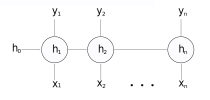
\includegraphics[width=0.5\textwidth]{pics/rnn_network}
  \caption{RNN for NER}
  \label{fig:rnn_network}
\end{figure}

At each timestep, the neural network computes a hidden state $ h_t $ using an input 
vector $ x_t $ and the previous hidden 
state $ h_{t-1} $, that retains information from past 
iterations. The input vector $ x_t $ for our RNN can consist of word features similar to 
the ones used in the previously discussed statistical models encoded in one-hot vectors,
word embeddings or a combination of both.
Finally, the RNN produces an output vector $ y_t $ representing the label for that 
timestep. A common definition for an RNN cell is given by the equations:

\begin{align*}
h_t &= tanh(W_x x_t + W_h h_{t-1}) \\
y_t &= softmax(W_y h_t)
\end{align*}

Where $ W_x $, $ W_h $ and $ W_y $ are weight matrices that can be trained with the 
Backpropagation Through Time (BPTT) algorithm. On a sequence labeling task, $ W_y $ 
is a $ |H| \times |Y| $ weight matrix where $ H $ is the size of the hidden layer,
defined experimentally according to the task, and $ Y $ is the number of classification labels
for our problem. With the softmax activation, the RNN will generate a probability distribution
across the range of possible labels and we can simply select the most probable label at each
timestep, assuming independence between labels. Theoretically, RNNs are capable of learning
and retaining long term dependencies with their internal state $ h_t $. However, in practice,
it becomes difficult due to the vanishing gradient problem. 

The vanishing gradient problem is one of the problems that we experience empirically that 
constrain theoretically sound network designs. When training neural networks, the weight 
updates are obtained from the partial derivatives of an error function 
(e.g. the cross-entropy). As these error derivatives are propagated to higher layers with
the chain rule, we have to multiply numbers that tend to get very small, so training becomes
less effective. This problem is particularly critical for RNNs, because we have constantly 
need to propagate weights through a relatively great number of timesteps.
Long short term memory networks (LSTM) were by~\cite{Hochreiter1997} with this problem in mind and 
they have been popularized since then. 

LSTMs incorporate a memory cell $ c $ in the RNN definition and three gates to control 
the flow of information that comes in and out of the memory cell.
The input gate $ \Gamma_{i} $ controls the amount of new information that will flow into the memory cell,
the forget gate $ \Gamma_{f} $ controls the amount of previous information that will be retained in the memory
cell, and the output gate $ \Gamma_{o} $ controls the amount of information stored in the memory cell that
will be used to compute the output activation of the LSTM unit. 
LSTM cell implementations vary slightly in the literature. A visual description of 
our LSTM cell is provided in Figure~\ref{fig:lstm_cell}.

\begin{figure}[h]
  \centering
  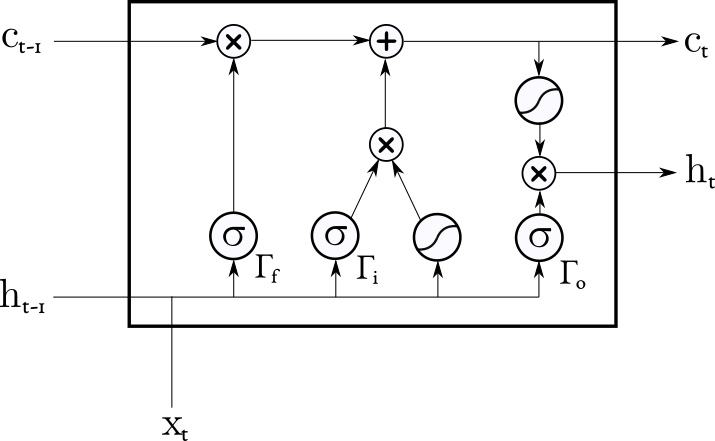
\includegraphics[width=0.5\textwidth]{pics/lstm_cell}
  \caption{LSTM Cell}
  \label{fig:lstm_cell}
\end{figure}

The equations for the LSTM cell are:

\begin{align*}
\Gamma_{i} &= \sigma(W_i \cdot [x_t,h_{t-1}] + b_i) \\
\Gamma_{f} &= \sigma(W_f \cdot [x_t,h_{t-1}] + b_f) \\ 
\Gamma_{o} &= \sigma(W_o \cdot [x_{t},h_{t-1}] + b_o) \\
c_t        &= \Gamma_{f} \ast c_{t-1} + \Gamma_{i} \ast tanh(W_c \cdot [x_{t},h_{t-1}] + b_c) \\
h_t        &= \Gamma_{o} \ast tanh(c_t)
\end{align*}

Where $ \sigma $ is the logistic sigmoid function. $ \Gamma_i $, $ \Gamma_f $, and $ \Gamma_o $ are the input,
forget and output gates, respectively, and $ W_i $, $ W_f $, $ W_o $ are the weight 
matrices corresponding to each gate. $ c_{t} $ is the cell 
state at time $ t $ and $ h_{t} $ is the hidden state at time $ t $. 
The vector $ [x_{t},h_{t-1}] $ is formed by concatenating the current input vector 
$ x_{t} $ and the hidden vector from a previous timestep $ h_{t-1} $. Finally,
$ A \ast B $ represents the element-wise multiplication of matrices $ A $ and $ B $
and $ A \cdot B $ represents the dot product of $ A $ and $ B $.


\subsection{BI-LSTM-CRF}
\label{sssec:lstm_crf}

On named entity recognition tasks, both past and future words are important 
to attribute a label at time $ t $, however a regular LSTM network only takes 
past states into consideration. A bidirectional LSTM solves this problem by stacking 
two regular LSTMs, and feeding them with observations in opposite directions. The first LSTM 
receives forward states and the second LSTM receives backward states. The hidden states from both 
networks can then be concatenated at each timestep to produce output labels. With this 
architecture, LSTM cells may use information from past and future timesteps to decide 
the label at time $ t $.

\cite{Huang2015} proposed a bidirectional LSTM with a CRF layer (BI-LSTM-CRF) on 
the output to tackle the sequence tagging problem. The main benefit of adding a CRF layer 
in the neural sequence model is that the labels are jointly decoded for a whole sentence 
instead of being predicted individually. Predicted tags should be highly correlated 
in a named entity recognition task, so it is desirable to predict sequences conjointly.
The BI-LSTM-CRF is described in Figure~\ref{fig:bi_lstm_crf}.

\begin{figure}[h]
  \centering
  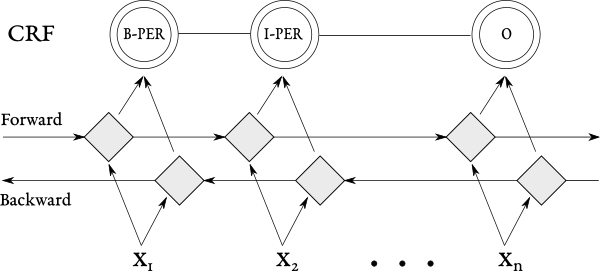
\includegraphics[width=0.5\textwidth]{pics/bi_lstm_crf}
  \caption{Bidirectional LSTM-CRF}
  \label{fig:bi_lstm_crf}
\end{figure}

This architecture achieved an F1 score of 90.10 on the English data from the CoNLL-2003 
NER shared task \cite{Sang2003}, in contrast to 85.17 for a bidirectional LSTM without 
a CRF layer. 


\subsection{Word Embeddings}

An important element of recurrent neural network architectures for text related tasks 
is the choice of word embeddings. Word embeddings are lower-dimensional representations of words in
continuous space. That is, each word is represented by a vector of continuous features (tipically a few hundred dimensions), 
often obtained with unsupervised clustering methods for words in large corpora. In comparison, one-hot encoded word 
vectors, that were popular before the introduction of word embeddings, are vectors with one dimension per 
word in the vocabulary (tipically a few hundred thousand dimensions) with 
zeros in all positions except for the index relative to that word. 

There are many advantages to the use of word embeddings relative to one-hot encodings. First, 
the number of weights learned by the sequence model is smaller because of the dimensionality
reduction. Second, the mapping of words into feature vectors makes possible the comparison of similarity 
between words according to their shared features. Finally, word embeddings 
can be pretrained without supervision on large corpora and be used on tasks for which there is 
little labeled data. 

Pretrained word embeddings are a powerful form of transfer learning, bootstrapping the learning 
of model parameters by first training it on a bigger dataset. 
This is especially useful in NER, because named entities that 
belong to the same class tend to have similar word embeddings. Thus, with good word embeddings, 
a neural network can predict the correct label for a word that was never seen during training
because it is similar to other words that occurred in the training set.

Pretrained word embeddings can also be further improved by fine tuning the feature values in the 
specific problem of sequence labeling, by allowing backpropagation to alter the embeddings. However, 
due to the limited size of most sequence labeling datasets, this technique ends up introducing
noise to the word representations instead of improving the word representations.

There are multiple methods that produce word embeddings, and most of the official implementations 
also provide pretrained word embeddings for the English language. In this work, we explored
three sets of pretrained embeddings: Word2Vec~\cite{Mikolov2013}, GloVe~\cite{Pennington2014} and 
ELMo~\cite{Peters2018}. The characteristics of each set of embeddings is given in 
Table~\ref{tab:word_embeddings}.

\begin{table}[h]
  \small
  \begin{center}
    \begin{tabular}{ lllll }
      \toprule
      Model & Dimensions & Training Set & Tokens (billions) & Vocab. \\
      \midrule
      Word2Vec & 300 & Google News & 100 & 3M   \\
      GloVe    & 300 & Gigaword5 + Wikipedia & 42 & 400K \\
      ELMo     & 512 & Wikipedia & 5.5 & - \\
      \bottomrule
    \end{tabular}
  \end{center}
  \caption{Model descriptions}
  \label{tab:word_embeddings}
\end{table}

Most breakthroughs in sequence labeling tasks in the past few years came through the introduction
of novel methods for constructing word embeddings. Different from earlier methods such as Word2Vec and
GloVe that produced static vectorial representations of words, more recent approaches such as
ELMo produce context dependent embeddings for a specific dataset with a neural network 
pretrained on a language modelling task. Also, the word representations in ELMo are entirely character based,
therefore there are no out-of-vocabulary words.

% As word embedding and language modelling methods become more sophisticated, it comes to mind
% if the complexity is entirely justifiable. 
% https://d4mucfpksywv.cloudfront.net/better-language-models/language_models_are_unsupervised_multitask_learners.pdf
% https://openai.com/blog/better-language-models/


\subsection{Character representations}

When devising deep neural architectures, one of the main objectives is to make the 
neural network discover useful features by itself instead of feeding it with what
we think is relevant. In NER, morphological features are very useful to classify
named entities. For example, knowing that the first character in a word is capitalized
means that it has a higher chance of being a proper name. We can add a character 
representation layer at the bottom of the Bi-LSTM-CRF to extract these morphological
features automatically. This way, we construct character representations, which are
fixed size morphological feature vectors, and concatenate them to the feature vectors $ x_t $
that were already being fed to the LSTMs. 

We describe below two methods to build character representations. Both of them receive 
character embeddings as inputs. Character embeddings are fixed size dense vectors that work
the same way as word embeddings, except that the lookup function maps characters to embeddings
instead of words to embeddings. This means that each word generates a character embedding 
matrix with size $ |W| \times |C| $, where $ |W| $ is the word length and $ |C| $ is the 
character embedding size (determined experimentally). Also, the character embeddings are 
trained in the target dataset instead of being trained in a larger corpus, since the vocabulary 
size is much smaller than in the case of word embeddings.


\subsubsection{CNN character representations}
\label{sssec:lstm_crf_cnn}

The CNN method proposed by~\cite{Ma2016} adds a convolutional neural network (CNN) layer 
on top of a bidirectional LSTM-CRF to encode character-level information. The CNN
layer is described visually in Figure \ref{fig:cnn}.

\begin{figure}[h]
  \centering
	  \includegraphics[width=0.5\textwidth]{pics/cnn}
  \caption{CNN-based character representations.}
  \label{fig:cnn}
\end{figure}

The convolutional neural network receives character embeddings as inputs and extracts
morphological features by sliding one dimensional filters over the sequence of characters 
and collapsing the filter outputs with a max pooling layer, producing a character
representation with a size determined by the number of filters. This means, that when a filter 
gets a good match at any position in the sequence, the max pooling layer output relative to that 
filter will be triggered, therefore this type of character representation detects position
invariant morphological features.


\subsubsection{LSTM character representations}

The LSTM method proposed by~\cite{Lample2016} models character-level 
representations on top of a Bi-LSTM-CRF similar to the one described in 
Figure~\ref{fig:bi_lstm_crf}, however instead of receiving words, it receives
sequences of character embeddings, then it combines the forward and backward 
LSTM hidden states to form the character representation, as described in 
Figure~\ref{fig:lstm_char}. 

\begin{figure}[h]
  \centering
  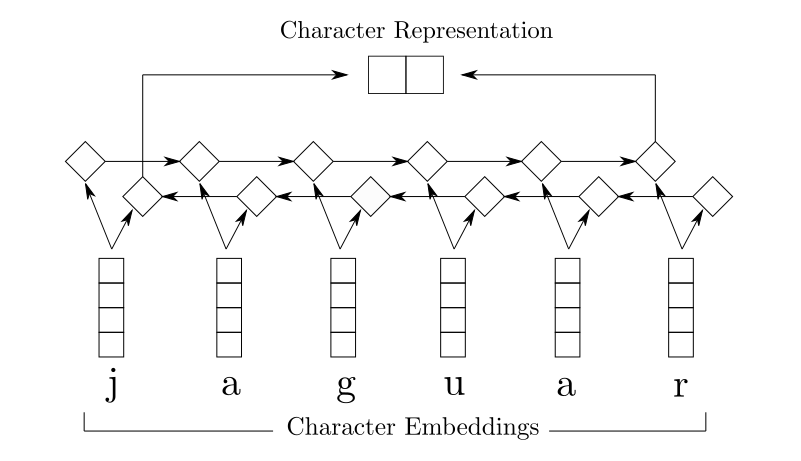
\includegraphics[width=0.5\textwidth]{pics/lstm_char_representations}
  \caption{LSTM-based character representations}
  \label{fig:lstm_char}
\end{figure}

The forward state is expected to be a better representation of the suffix of 
a token, and the backward state is expected to be a better representation of 
the prefix of a token. This differentiates the architecture
from the CNN method, because CNN filters discover positional invariant features, 
while LSTMs can better represent suffixes and prefixes. 


\subsection{Conclusion}

Eventhough word embeddings and character representations can make up for the feature engineering 
that was required by earlier statistical approaches to sequence labeling, there are still some
technical concerns to be faced that require quite a bit of engineering. The loss functions that need
to be optimized by our neural architectures is not convex, therefore the choice of the optimization 
function can impact the resulting set of parameters for our model as well as the hyperparameter choice 
for these functions. Neural networks are also prone
to overfitting, what can be partially avoided with the addition of dropout layers as in~\cite{Srivastava2014}
or with the early stopping strategy over a validation dataset as in~\cite{Caruana2000}. 

Another difficulty in training neural networks comes from the training time required for convergence
to a good set of parameters. This sometimes requires the employment of expensive hardware,
layer normalization and parallelization strategies. All of this adds into the complexity, hardware cost 
and training cost of our models, many times providing only slight 
improvements over simpler approaches. 


\section{Summary}

In this chapter we introduced multiple models for sequence labeling and, particularly,
NER. In Section~\ref{sec:hmm}, we presented Hidden Markov Models, a generative model for 
sequence labeling that can be derived with probability theory if we consider that
text has the properties of a Markov sequence. In Section~\ref{sec:crf}, we discussed
Conditional Random Fields, a discriminative analogue to HMMs that relaxes some 
assumptions made by HMMs and allows the usage of overlapping feature functions in
context vectors. Finally, in Section~\ref{sec:neural_networks}, we discussed Neural Networks
for sequence labeling, the state-of-the-art approach. Contrasting with the earlier statistical
approaches, neural models are more empirically oriented and much more complex in terms of
the number of parameters and the time required for convergence during training.


\chapter{Sequence Labeling on the Web}

In the last chapter, we discussed sequence models that can be generally employed in 
a diverse range of natural language processing tasks. However, there are some specificities 
to the problem of sequence labeing on the web that can be explored to allow further improvement 
of our models. In Section~\ref{sec:self_training}, we introduce the self-training strategy
for Hidden Markov Models. In Section~\ref{sec:attention_models}, we introduce two attention models
to incorporate HTML structural information in our neural sequence taggers. In
Section~\ref{sec:fscore_optimization}, we propose a new optimization objective for neural 
networks trained for sequence labeling tasks.


\section{Self-Training for Hidden Markov Models} 
\label{sec:self_training}

As described in Section~\ref{sec:hmm}. The simplest conceivable Hidden Markov Model 
for the sequence labeling on HTML task is a generative classifier that has the form:

\begin{equation}
P(X,Y) \propto \prod_{i=1}^n P(x_i|y_i) P(y_i, y_{i-1})
\end{equation}

Where $ X $ is a sequence of words and $ Y $ is a sequence of labels, both with size $ n $,
and the initial probabilities $ P(y_1|y_0) $ are uniform across all label assignments.
To construct this model from the data, we need to estimate the probabilities:

\begin{itemize}
  \item $ P(x_i|y_i) $: the emission probability of word $ x_i $ given label $ y_i $.
  \item $ P(y_i|y_{i-1}) $: the transition probability of going to label $ y_i $ from label $ y_{i-1} $.
\end{itemize}

We may consider $ x_i $ to be a binary feature vector $ x_i = \{ f_{i,1}, f_{i,2}, ..., f_{i,k} \} $
as long as all the feature distributions are independent, conditioned on $ y_i $. That is:

\begin{equation}
P(x_i|y_i) = P(f_{i,1}, f_{i,2}, ..., f_{i,k}|y_i) = \prod_{j=1}^k P(f_{i,j}|y_i)
\end{equation}

With this assumption, we can obtain the maximum likelihood estimators for feature parameters
from their relative frequencies, just as we did in Section~\ref{sec:hmm} for single words 
(Equation~\ref{eq:mle_words}). Then, for binary features:

\begin{equation}
\hat{P}(f_{i,j}=1|y_i=L) = \frac{\text{Count}(f_{*,j}=1, y_*=L)}
{\text{Count}(f_{*,j}=0, y_*=L) + \text{Count}(f_{*,j}=1, y_*=L)}
\label{eq:feature_mle}
\end{equation}

The $ * $ symbol means for every assignment of $ i $, because the probabilities are time invariant.
This approach yields good experimental results for textual features such as the capitalization
of a word, but if we try to use HTML structural features such as the HTML tags, we will find that
they are not very useful, contradicting our intuition.
The problem is that there is not much statistical similarity between the HTML structure in different web pages.
For example, only because a named entity label occurs more often inside <div> tags
in a page, that does not mean this is the case for most web pages. Consider for example a faculty web page 
that shows researcher names in a table (<td> tags) in contrast to a web page that organizes researcher
names in a list (<li> tags). If the first page is in our training set, and we use the HTML tag feature to 
assign labels to the second page in our test set, we will probably get many wrong predictions.
Nonetheless, the HTML features are not useless. Inside a single web page, the HTML tag is a good predictor
of the correct labels. Words with a similar HTML context tend to have similar labels. The question
is how to obtain better parameter estimators for HTML features.

Consider a set of $ m $ textual features unrelated to the HTML structure:

\begin{equation*}
F^T = \{ f^T_1, f^T_2, ..., f^T_m \}
\end{equation*}

And a set of $ k $ HTML features that are related to the HTML structure:

\begin{equation*}
F^H = \{ f^H_1, f^H_2, ..., f^H_k \}
\end{equation*}

Given a Hidden Markov Model $ H^T $ trained with only the first set of features $ F^T $,
we can use $ H^T $ to predict the labels of an unlabeled document, and then we simply replace 
the actual labels in Equation~\ref{eq:feature_mle} with the predicted labels $ \tilde{Y} $:

\begin{equation}
\hat{P}(f_{i,j}=1|y_i=L) = \frac{\text{Count}(f_{*,j}=1, \tilde{y}_*=L)}
{\text{Count}(f_{*,j}=0, \tilde{y}_*=L) + \text{Count}(f_{*,j}=1, \tilde{y}_*=L)}
\end{equation}

Next, we incorporate the estimators for the HTML feature probabilities in $ H^T $ and predict
the final labels with the whole set of features $ F^T \cup F^H $. This self-training
strategy can be implemented like this:

\begin{itemize}
\item Train the HMM without any HTML features.
\item Compute labels for a website with the trained HMM.
\item Use the computed labels as a proxy for the actual labels in the 
website and estimate HTML feature frequencies for this website alone.
\item Recompute the labels now using the HTML feature probabilities.
\end{itemize}

This strategy could possibly be incorporated in the Baum-Welch algorithm, but this heuristic
approach already yields a consistent improvement to sequence labeling on the web. In theory, this 
strategy could be used with any sequence tagger, however retraining a classifier with new features can 
become prohibitively expensive in the case of CRFs or neural networks. In HMMs, retraining the features
is really fast, because we assume feature independence and the maximum likelihood estimator can be obtained
with a simple closed form expression.


\section{Attentions Models} 
\label{sec:attention_models} 

The self-training strategy for HMMs demonstrates a way to incorporate HTML features in 
sequence models, however it is not clear how to apply the same intuition to neural 
networks. Ultimately, we want the model to consider the predictions that it made for 
words in similar HTML contexts when constructing the neural representation for the 
current word in a sequence. A natural way to incorporate this intuition into the neural 
architectures described in Section~\ref{sec:neural_networks} is with the use of 
self-attention mechanisms, created by~\cite{Vaswani2017}.
Originally, attention mechanisms were developed with the goal of solving sentence alignment 
for neural machine translation in~\cite{Bahdanau2014}, but since then it
found other uses in NLP. An attention mechanism is a way to combine
inputs from multiple timesteps in a sequence to perform an operation at the current timestep.

In a LSTM-CRF model, the bidirectional LSTM layer produces output representations at each 
timestep, producing a $ T \times H $ matrix, where $ T $ is the number of timesteps in the
sequence and $ H $ is the LSTM hidden layer size, which is defined arbitrarily (we omit
the batch size in this matrix representation). If the sequence length in the dataset varies,
we can simply pad the short sentences with zero vectors. In other words, this matrix
constitutes a neural representation for a sentence with vectors of size $ H $ representing
words at each timestep. In the original LSTM-CRF model without an attention layer, these
neural representations would be passed directly to the CRF decoder, but in the Self-Attended 
Bi-LSTM-CRF, we add an attention mechanism between the LSTM output and the CRF input as described 
in Figure~\ref{fig:lstm_attention}.

\begin{figure}[h]
  \centering
  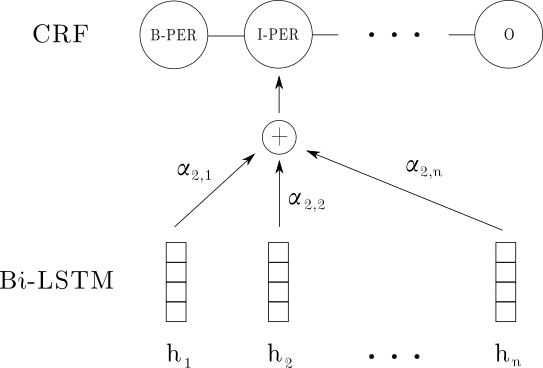
\includegraphics[width=0.5\textwidth]{pics/lstm_attention}
  \caption{Attention mechanism for the Bi-LSTM-CRF model.}
  \label{fig:lstm_attention}
\end{figure}

Now we need to find a way to combine the vectors at each timestep in a way that transforms 
the representations according to the similarity between HTML contexts. Essentialy, we want to compute a $ T \times T $ 
attention matrix $ \alpha $ where $ \alpha_{i, j} $ is the weight attributed to the word representation $ h_j $ at timestep
$ i $. In other words, $ \alpha_{i, j} $ is measuring the amount of attention that we pay to each word $ j $ in
a sentence at timestep $ i $. With the $ \alpha $ matrix, we can calculate new representations $ h'_i $ 
for each timestep by performing a linear combination of the hidden states according to their 
attention values:

\begin{equation}
h'_i = \sum_{j} = \alpha_{i, j} h_j
\end{equation}

Also, consider a set of $ n $ context vectors $ c_i $ that contain representations for the
html features at timestep $ i $. This representation can be a binary feature vector,
a dense vector or even the hidden states $ h_i $. The attention matrix is then calculated as:

\begin{equation}
\alpha_{i,j} = \frac{e^{A(c_i, c_j)}}{\sum_k e^{A(c_i, c_k)}}
\end{equation}

Where $ A(c_i, c_j) $ is an attention function that computes the similarity between
HTML contexts at timesteps $ i $ and $ j $ and outputs a real number. The exponentials are
a softmax normalization function to ensure that $ 1 \geq \alpha_{i,j} \geq 0 $ and 
$ \sum_{j} \alpha_{i, j} = 1 $. Next we propose two ways for defining the attention function
$ A $. The Hard Attention Function and the Soft Attention Function. 

\subsection{Hard Attention Function}

The hard attention function is a binary similarity function that either outputs one when 
contexts are identical or zero when they are different. This definition only makes sense
when the contexts $ c_i $ at timestep $ i $ are discrete feature vectors, because otherwise 
we would need a softer comparability criterion. So, if $ c_i = \{ f_{i,1}, f_{i,2}, ..., f_{i,m} \} $
is a context vector where each feature $ f_{i,j} $ assumes a definite value from a discrete set
$ \gamma_j $, we can define the attention function:

\begin{equation}
  A(c_i, c_j) = \begin{cases} 
    1, \text{ if } f_{i,k} = f_{j,k} \;\;\; \forall \; k \in [1,m] \\ 
    0, \text{ otherwise}
  \end{cases}
\end{equation}

The combination of features must be sufficiently restrictive so that the mixture of hidden
states does not introduce too much noise. We have determined experimentally that considering
only three features: the enclosing HTML tag, its parent tag and the CSS class; is sufficient to 
allow a consistent comparison between similar HTML contexts. Ideally, the choice of features
could be performed automatically with the incorporation of a feed forward neural network in
the comparison function and a softer similarity criterion. A possibility for doing this is 
the Soft Attention Function.


\subsection{Soft Attention Function}

Different from the Hard Attention Function, the Soft Attention Function outputs a real number 
that represents the degree of similarity between HTML contexts. Now, instead of considering
discrete feature vectors we resort to dense vectorial representations for the HTML context.
Similar to the way we extracted morphological features with characters representations in
Section~\ref{ssec:char_representations}, we can extract HTML structural features with
DOM path representations. To do this, consider a DOM tree (which is an acyclic directed graph),
a word's HTML context can be represented by the path we take in this graph starting from the 
root element. If we consider the path for each word in our sequence, we can create HTML dense 
representations by training a matrix of fixed size embeddings for each HTML tag, then we construct 
HTML representations by averaging the embeddings in a final vector representation. The process
is described in Figure~\ref{fig:html_embeddings}. 

\begin{figure}[h]
  \centering
  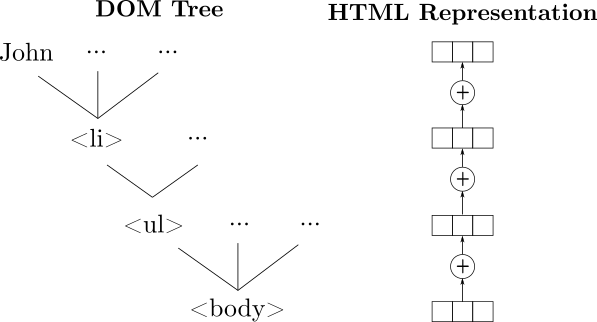
\includegraphics[width=0.5\textwidth]{pics/html_embeddings}
  \caption{Building HTML representations by climbing the DOM tree.}
  \label{fig:html_embeddings}
\end{figure}

Experimentally, we only considered the last two HTML embeddings, since the HTML tag 
information gets less relevant as we get farther from the leaves. The vocabulary of HTML 
tags is very small, so we can train HTML embeddings effectively in the target dataset. 
We could also learn HTML representations with CNNs or LSTMs as we did with character 
representations, instead of averaging the embeddings. 

Now to measure the similarity between different HTML contexts, we resort to an attention
function similar to the scaled dot product proposed by~\cite{Vaswani2017}. That is:

\begin{equation}
  A(c_i, c_j) = \frac{W c_i \cdot W c_j}{\sqrt{n}}
\end{equation}

Where $ W $ is a weight matrix to be learned and $ \sqrt{n} $ is a normalization factor
with $ n $ being the size of the context vectors $ c $. This function assumes a larger
value when the contexts are similar and a smaller value when they are different. With the 
soft attention mechanism, our model can learn HTML context representations from the training 
data and generalize patterns such as: if some words happen together in a list then they probably 
belong to the same class.


\subsection{Dataset split and Experimental Considerations}

In sequence labeling tasks, it is common to split the dataset in sentences and then train them
in independent steps. However, if we want to make use of attention mechanisms to 
perform the comparison of words in different HTML contexts, we want to compare labels attributed 
to words that share a similar context in different sentences. 
To allow the comparison of words in different sentences, instead of splitting the dataset into
independent shuffled sentences, we combined multiple sentences in a single training step and separated 
them with a segmentation token. Also, with the addition of many parameters to the model, the risk of 
overfitting increases. To prevent this problem from occurring, we added dropout layers with a 0.5 
dropout rate before and after the attention mechanism.


\section{F-measure Optimization} 
\label{sec:fscore_optimization}

In the LSTM-CRF model, we estimate parameters by maximizing the log-likelihood. The likelihood is 
intimately associated with the accuracy in a classification task, but in NER tasks, models are 
usually evaluated according to their Precision, Recall, or their harmonic mean (i.e. the F-measure).
By maximizing the likelihood, we are essentialy increasing acccuracy with the expectation that this 
will lead to an improvement of the F-measure, what is most often true. However, there is a trade-off 
between Precision and Recall, meaning that we can trade a little less Precision for an increase in
Recall and vice-versa.

In NER on HTML, we could argue that Recall is slightly more important than Precision, because when 
we are parsing a huge amount of data, it is much easier to manually filter false positives than 
manually finding the false negatives that were ignored by the classifier. This preference for Recall
could be expressed in our evaluation by setting the F-measure $ \beta $ in a way that values Recall twice 
as much as Precision, for example. However, when maximizing the accuracy of a classifier
with the cross-entropy function, we have no way to tell the optimizer to choose the parameters that maximize 
the F-measure with a particular $ \beta $. We could try to maximize the F-measure directly, but:

\begin{quote}
While the F-measure of a classifier evaluated on a single supervised instance is well defined, the
overall F-measure on a larger dataset is not a function of the F-measure evaluated on each instance
in the dataset. This is in contrast to ordinary loss/utility, whose grand total (or average) on a dataset
can be computed by direct summation~\cite{Jansche2005}.
\end{quote}

This makes the usage of the F-measure as an optimization objective impractical for large datasets trained in 
batches. However, with a few simplifications, we can replace our loss function and instead 
maximize the F-measure in terms of the expected utility. We take the method proposed by~\cite{Jansche2005}, that
approximately maximizes the F-measure of a classifier based on a logistical regression model, and 
apply it on our neural architectures. The F-measure function can be calculated in terms of a triple (A,B,C):

\begin{equation}
F_\alpha(A, B, C) = \frac{A}{A + \alpha B + (1-\alpha) C}
\end{equation}

This is equivalent to the $ \beta $-weighted harmonic mean defined in Equation~\ref{eq:fscore_formula}.
Variable $ A $ is the number of true positives, $ B $ is the number of false negatives, and $ C $ is the number 
of false positives. Also, consider that:

\begin{eqnarray*}
n_{pos} = A + B \\
m_{pos} = A + C
\end{eqnarray*}

That is, $ n_{pos} $ is the number of positive examples in the dataset (true positives plus missed positives) 
and $ m_{pos} $ is the number of positive examples that were predicted (true positives plus false positives).
With this, we can rewrite $ F_\alpha(A, B, C) $ as:

\begin{equation}
F_\alpha(A, B, C) = \frac{A}{\alpha n_{pos} + (1-\alpha) m_{pos}}
\end{equation}

With this expression in mind, \cite{Jansche2005} proposes the optimization objective:

\begin{equation}
\tilde{F}_\alpha(\hat{y}, y) = 
  \frac{\tilde{A}(\hat{y}, y)}
  {\alpha \tilde{n}_{pos} + (1-\alpha) \tilde{m}_{pos}(\theta)}
\end{equation}

Where $ \hat{y} = \{ \hat{y}_1, \hat{y}_2, \ldots, \hat{y}_n \} $ is a vector of predictions,
$ y = \{ y_1, y_2, \ldots, y_n \} $ is a vector with the actual labels, and:

\begin{equation}
\theta_i \equiv \hat{P}(y_i = \textit{True}) \;\; \forall i \; \in \; [1, n]
\end{equation}

That is, $ \theta_i $ is the probability attributed by the model that the label at time $ i $ is a
\textit{True} label, assuming that we are dealing with a binary classification 
problem with only \textit{True} and \textit{False} labels. Finally:

\begin{align*}
\tilde{A}(y, \hat{y}) & \equiv \sum_{i=1}^n I_{y = \hat{y} = 1} \cdot \theta_i  \\
\tilde{m}_{pos}       & \equiv \sum_{i=1}^n \theta_i \\
\tilde{n}_{pos}       & \equiv \sum_{i=1}^n I_{y=1} - \tilde{A}(y, \hat{y})
\end{align*}

Where $ I_{Z} $ is an identity function that is one when the clause $ Z $ is true and zero otherwise.
With that, we have defined an optimization objective that can be optimized with standard numerical optimization methods.
Different from the actual F-measure employed on a sequence labeling problem, we consider that each label here 
is independent and belongs to a different entity. Further work is needed to resolve this simplification and to 
adapt this optimization function to multi-label classification tasks. But, as we will see in the experiments section,
this formulation is sufficient for the researcher name extraction task.

\section{Summary}

In this chapter we have discussed several methods for improving the performance of sequence
labeling models in NER on HTML. Section~\ref{sec:self_training} and Section~\ref{sec:attention_models} 
discussed methods for incorporating HTML features in Hidden Markov Models and Neural Networks. 
Section~\ref{sec:fscore_optimization} discussed the usage of a modified F-measure function as
an optimization objective for neural networks to allow the choice of specific Precision or Recall 
goals.


\chapter{Experiments}
\label{cha:experiments}

The main objective of this dissertation is to find the best method for performing NER on the 
web considering the researcher name extraction task. The value of a specific method is determined
not only by its accuracy, but also by the amount of feature engineering required, the training
time required, and the overall complexity of the model when we consider its gains relative to
simpler alternatives. With this objective in mind, we pose the following research questions:

\begin{enumerate}

\item Are Hidden Markov Models effective for solving the researcher name extraction task?
\begin{enumerate}
\item Does the order of the Hidden Markov Model influence its performance?
\item Can we improve a HMM by adding textual features?
\item Can we improve a HMM with the self-training strategy?
\end{enumerate}

\item Are Conditional Random Fields effective for solving the researcher name extraction task?
\begin{enumerate}
\item Are featureless linear chain CRFs better than featureless HMMs?
\item Can we improve the CRFs by adding textual features?
\item Are CRFs more resilient to bad features than HMMs?
\end{enumerate}

\item Are Neural Networks effective for solving the researcher name extraction task?
\begin{enumerate}
\item How does a featureless LSTM-CRF compare with HMMs and CRFs?
\item Can character representations boost the performance of the Bi-LSTM-CRF?
\item Does the selection of word embeddings influence the performance of the Bi-LSTM-CRF?
\item Can the hard-attention and soft-attention mechanisms boost the performance of the Bi-LSTM-CRF?
\item Can we control how much the Bi-LSTM-CRF values recall over precision by changing the optimization objective?
\end{enumerate}

\item All things considered what is the best model?
\begin{enumerate}
\item What model has the best F1-score?
\item Can we improve the results of the best models with a simple filtering strategy?
\item What do we lose and what do we gain as we increase the complexity of the models?
\end{enumerate}

\end{enumerate}

All models in this dissertation were trained and tested in the dataset described in Chapter~\ref{cha:dataset}.
When relevant, the technical specifications for the experiments will be given in each section.
Section~\ref{sec:baseline} establishes a featureless baseline in addition to the dictionary
matching baseline that was described in Chapter~\ref{cha:dataset} for the researcher name
extraction task. Section~\ref{sec:experiments_hmm} discusses the experimental results that concern
Research Question 1. Section~\ref{sec:experiments_crf} discusses the experimental results that 
concern Research Question 2. Section~\ref{sec:experiments_nn} discusses the experimental results 
that concern Research Question 3. Finally, Section~\ref{sec:experiments_best} discusses the experimental 
results that concern Research Question 4.


\section{Simple Baseline}
\label{sec:baseline}

A model that works well despite the absence of a good feature selection is more valuable than
a method that requires a lot of feature engineering or a model that requires a big dictionary of
named entities. For this reason, we wanted to establish some baseline results in addition to 
the gazetteer matching results presented in Chapter~\ref{cha:dataset}. For this purpose, we
trained a simple generative model and a simple discriminative model to provide a measure of the
expected difficulty of solving this task. The simple generative model is a Naive Bayes classifier,
which is essentialy a \textit{Hidden Markov Model}, as presented in Section~\ref{sec:hmm}, with the
assumption of label independence. That is, $ P(Y_i|Y_{i-1}) = P(Y_i) $ for all timesteps $ i $. 
The simple discriminative model is a Logistic Classifier, as presented in Section~\ref{sec:crf}. 

The "Naive-Bayes and Logistic Classifiers form a generative-discriminative pair"~\cite{Ng2001},
in the sense that the essential difference between the models is that the first estimates the
joint probability between words and labels $ P(X, Y) $ and the latter models the conditional
probability $ P(Y|X) $. The same analogy can be made for HMMs and CRFs. The Naive Bayes model and
the Logistic Classifier are very simple and fast to train, so they provide a good 
first approximation to a solution for this task. Both models used only the current word as a
feature. Table~\ref{tab:nb_and_maxent} shows a comparison between these models and the dictionary
matching approach.

\begin{table}[h]
  \small
  \begin{center}
    \begin{tabular}{ lllllll }
      \toprule
      \multirow{2}{*}{Model} & \multicolumn{3}{c}{Validation} & \multicolumn{3}{c}{Test} \\
                             & \multicolumn{1}{c}{P} & \multicolumn{1}{c}{R} & \multicolumn{1}{c}{F1}
                             & \multicolumn{1}{c}{P} & \multicolumn{1}{c}{R} & \multicolumn{1}{c}{F1} \\
      \midrule
      Gazetteer Matching     & 0.847 & 0.285 & 0.427 & 0.871 & 0.328 & 0.477          \\
      Naive Bayes            & 0.172 & 0.851 & 0.287 & 0.181 & 0.776 & 0.294          \\
      Maxent                 & 0.287 & 0.547 & 0.377 & 0.335 & 0.508 & 0.404          \\
      \bottomrule
    \end{tabular}
  \end{center}
  \caption{Naive Bayes and Logistic Classifier in the researcher name extraction task.}
  \label{tab:nb_and_maxent}
\end{table}

As previously discussed, the Maximum Entropy classifier allows for overlapping features while
the Naive Bayes assumes feature independence. That is possibly why the Logistic Classifier 
performs better than the Naive Bayes model in this problem. However, both models are worse than 
the dictionary matching approach when we consider the F1-score. With these baselines we can
proceed to test more complex models.


\section{Hidden Markov Models}
\label{sec:experiments_hmm}

There are a couple of parameters that need to be considered when we employ \textit{Hidden Markov Models}
in a sequence labeling task. First, the number of previous states (the order of the HMM) and, second, 
the model features.

\subsection{HMM order}

We hypothesized that the performance of HMMs on sequence labeling tasks for NLP can be improved by
raising the number of previous states checked at each timestep, that is the order of the HMM.
Table~\ref{fig:hmm_no_features} shows the performance of \textit{HMMs} up to third 
order in the test sets of the NER on HTML dataset. To allow comparison with the baselines, we also 
add the results of a Naive Bayes classifier. The Naive Bayes classifier can be thought of as a
HMM of zeroth-order.

\begin{figure}[h!]
  \begin{center}
    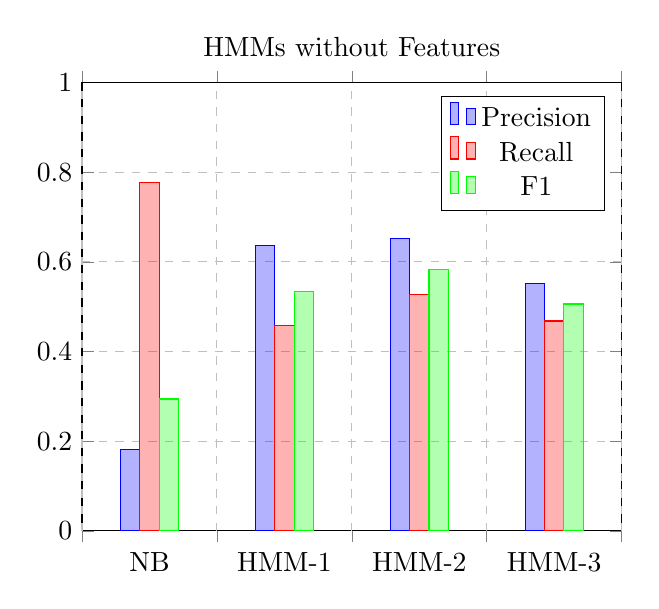
\begin{tikzpicture}
      \begin{axis}[
        title={HMMs without Features},
        xmin=0.5, xmax=4.5,
        ymin=0, ymax=1,
        xticklabels={NB,HMM-1,HMM-2,HMM-3},
        xtick={1,...,4},
        ytick={0,0.2,...,1},
        ybar=0pt,
        bar width=7pt,
        xtick distance=1,
        xtick style={
            /pgfplots/major tick length=0pt,
        },
        extra x ticks={-0.5,0.5,...,5.5},
        extra x tick labels=\empty,
        extra x tick style={
            grid=major,
            xtick style={
                /pgfplots/major tick length=4pt,
            },
        },
        ymajorgrids=true,
        grid style=dashed,
        legend pos=north east,
      ]

      \addplot[ybar, color=blue, fill=blue, fill opacity=0.3,] coordinates {
        (1,0.181)(2,0.637)(3,0.653)(4,0.551)
      };
      \addplot[ybar, color=red, fill=red, fill opacity=0.3,] coordinates {
        (1,0.776)(2,0.458)(3,0.527)(4,0.468)
      };
      \addplot[ybar, color=green, fill=green, fill opacity=0.3,] coordinates {
        (1,0.294)(2,0.533)(3,0.583)(4,0.506)
      };
      \legend{Precision, Recall, F1};
       
      \end{axis}
    \end{tikzpicture}
    \caption{
      Performance of the Naive Bayes classifier and Hidden Markov Models without 
      features besides the current word on the test set of the NER on HTML dataset.
    }
    \label{fig:hmm_no_features}
  \end{center}
\end{figure}

Considering label dependencies over multiple timesteps increases the classifier performance by a considerable margin 
relative to the Naive Bayes model even without the addition of any features besides the current word. The 
second order HMM (HMM-2) achieved an F1-score of 0.583 at the task, while
the Naive Bayes classifier achieves an F1-score of 0.294 and the dictionary matching approach 
only achieved an F1-score of 0.477. Nevertheless,
we already observe a relative decline in performance with the third order \textit{HMM} (0.506 F1-score), 
suggesting that increasing the order of the \textit{HMM} is not always advantegeous. This is probably because
as we increase the window of previous labels at each timestep, the label combinations get less common
in the training set, and therefore, the probability estimates get less reliable.


\subsection{Feature selection}

Eleven categorical features were extracted from the dataset. 
These were selected through feature engineering from a larger pool of features, 
considering their aid to the performance of the extraction systems. Deep learning 
architectures can work incredibly well without any of these features, however they
are of critical importance to traditional approaches such as HMMs and CRFs. 
The selected features are presented in Table~\ref{tab:features}. 

\begin{table}[h]
  \small
  \begin{center}
    \begin{tabular}{ ll }
      \toprule
      Feature & Description \\
      \midrule
      1  & Unaccented lowercase token \\
      2  & Exact gazetteer match \\
      3  & Partial gazetteer match \\
      4  & Email \\
      5  & Number \\
      6  & Honorific (Mr., Mrs., Dr., etc.)\\
      7  & Matches a URL \\
      8  & Is capitalized \\
      9  & Is a punctuation sign \\
      10 & HTML tag + parent \\
      11 & CSS class \\
      \bottomrule
    \end{tabular}
  \end{center}
  \caption{Features used in the NER-on-HTML dataset}
  \label{tab:features}
\end{table}

\begin{description}
\item[Feature 1] is the token converted to unaccented lowercase format.
\item[Feature 2] represents an exact match of a sequence of tokens to any of the 1,595,771 
names from the dictionary extracted from DBLP described in Section~\ref{sec:dictionary}.
\item[Feature 3] represents a partial match in the same dictionary. 
\item[Feature 4] is a binary feature describing a regular expression match to an email address.
\item[Feature 5] is true if the token contains a number.
\item[Feature 6] is true if the token is an honorific.
\item[Feature 7] is true if the token matches the regular expression for a URL.
\item[Feature 8] is true if the token is capitalized.
\item[Feature 9] is true if the token is a punctuation sign.
\item[Feature 10] is the token's enclosing HTML tag and its parent tag concatenated.
\item[Feature 11] is the CSS class for the token's HTML tag.
\end{description}

Features 10 and 11 are only useful in the self-training strategy for HMMs and the
attention architectures for Bi-LSTM-CRFs.
We know that correlated features may hurt the performance of some classifiers, so
in Table~\ref{tab:feature_correlation} we present the feature correlation matrix based on 
the Cram�r's V measure.
% ~\footnote{
% Dpython implementation
% % https://en.wikipedia.org/wiki/Cram%C3%A9r%27s_V
% % https://github.com/shakedzy/dython/blob/master/dython/nominal.py
% }. 

\begin{table}[h]
  \tiny
  \begin{center}
    \begin{tabular}{ lccccccccccc }
      \toprule
           & \rot{Word} & \rot{Exact Match} & \rot{Partial Match} & \rot{Email} & \rot{Number} & \rot{Honorific} 
	   & \rot{URL} & \rot{Capitalized} & \rot{Punctuation} & \rot{HTML Tag} & \rot{CSS Class} \\
      \midrule
      Word          & 1.00 & \textbf{0.60} & \textbf{0.94} & \textbf{1.00} & \textbf{1.00}  & \textbf{1.00} & 0.00 & \textbf{0.84} & \textbf{1.00}  & 0.25 & 0.00 \\
      Exact Match   & -    & 1.00  & 0.19  & -0.02 & -0.07 & -0.04 & 0.00 & 0.15  & -0.05 & 0.07 & 0.22 \\
      Partial Match & -    & -     & 1.00  & -0.11 & -0.35 & -0.09 & 0.00 & -0.01 & 0.45  & 0.04 & 0.17 \\
      Email         & -    & -     & -     & 1.00  & -0.02 & -0.02 & 0.00 & -0.12 & -0.05 & 0.03 & 0.27 \\
      Number        & -    & -     & -     & -     & 1.00  & -0.07 & 0.00 & -0.36 & -0.16 & 0.09 & 0.34 \\
      Honorific     & -    & -     & -     & -     & -     & 1.00  & 0.00 & 0.15  & -0.08 & 0.02 & 0.11 \\
      URL           & -    & -     & -     & -     & -     & -     & 1.00 & 0.00  & 0.00  & 0.00 & 0.00 \\
      Capitalized   & -    & -     & -     & -     & -     & -     & -    & 1.00  & -0.48 & 0.07 & 0.28 \\
      Punctuation   & -    & -     & -     & -     & -     & -     & -    & -     & 1.00  & 0.04 & 0.11 \\
      HTML Tag      & -    & -     & -     & -     & -     & -     & -    & -     & -     & 1.00 & \textbf{0.64} \\
      CSS Class     & -    & -     & -     & -     & -     & -     & -    & -     & -     & -    & 1.00 \\
      \bottomrule
    \end{tabular}
  \end{center}
  \caption{Feature correlation matrix}
  \label{tab:feature_correlation}
\end{table}

The current word is strongly correlated with most features besides the URL feature, and the ones related to 
the HTML structure. That shows there is not a lot of information to gain from these features. To understand how
this can help or hurt the Hidden Markov Model performance we test the model using two groups of features:

\begin{description}
  \item[Group A] Current word, Exact Match, Partial Match, URL, Capitalized
  \item[Group B] All features except HTML Tag and CSS Class
\end{description}

Group A is composed of features with a smaller correlation and Group B is composed of all 
textual features. Figure~\ref{fig:hmm_features} compares the performance of HMMs using the 
features from Group A and Group B. 

\begin{figure}[h!]
  \begin{center}
    \tiny
    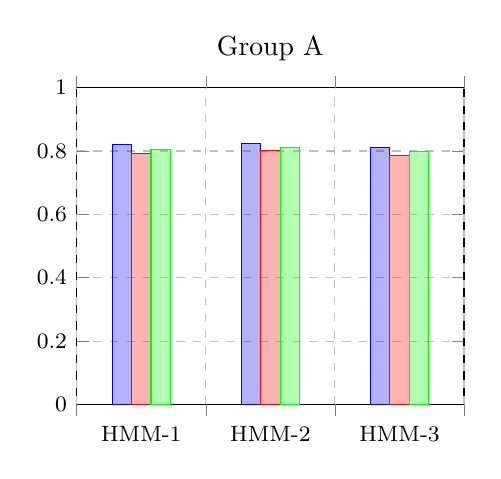
\begin{tikzpicture}
      \pgfplotsset{small}
      \begin{axis}[
        title={Group A},
        xmin=0.5, xmax=3.5,
        ymin=0, ymax=1,
        xticklabels={HMM-1,HMM-2,HMM-3},
        xtick={1,...,3},
        ytick={0,0.2,...,1},
        ybar=0pt,
        bar width=7pt,
        xtick distance=1,
        xtick style={
            /pgfplots/major tick length=0pt,
        },
        extra x ticks={-0.5,0.5,...,5.5},
        extra x tick labels=\empty,
        extra x tick style={
            grid=major,
            xtick style={
                /pgfplots/major tick length=4pt,
            },
        },
        ymajorgrids=true,
        grid style=dashed,
      ]

      \addplot[ybar, color=blue, fill=blue, fill opacity=0.3,] coordinates {
        (1,0.819)(2,0.823)(3,0.812)
      };
      \addplot[ybar, color=red, fill=red, fill opacity=0.3,] coordinates {
        (1,0.792)(2,0.802)(3,0.785)
      };
      \addplot[ybar, color=green, fill=green, fill opacity=0.3,] coordinates {
        (1,0.805)(2,0.812)(3,0.798)
      };
      \legend{};
       
      \end{axis}
    \end{tikzpicture}
    ~
    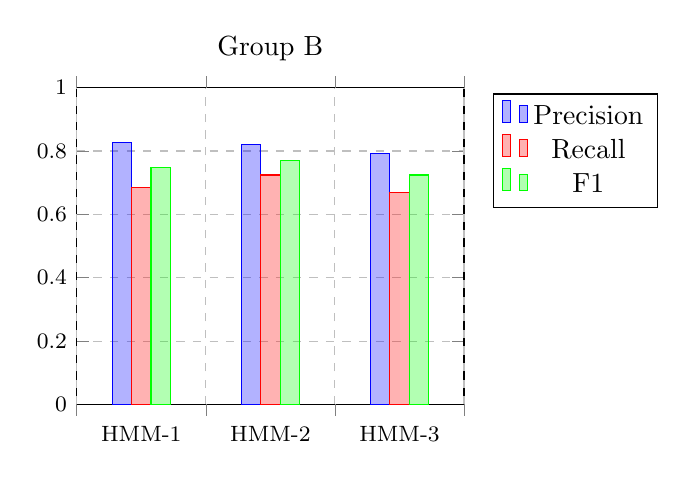
\begin{tikzpicture}
      \pgfplotsset{small}
      \begin{axis}[
        title={Group B},
        xmin=0.5, xmax=3.5,
        ymin=0, ymax=1,
        xticklabels={HMM-1,HMM-2,HMM-3},
        xtick={1,...,3},
        ytick={0,0.2,...,1},
        ybar=0pt,
        bar width=7pt,
        xtick distance=1,
        xtick style={
            /pgfplots/major tick length=0pt,
        },
        extra x ticks={-0.5,0.5,...,5.5},
        extra x tick labels=\empty,
        extra x tick style={
            grid=major,
            xtick style={
                /pgfplots/major tick length=4pt,
            },
        },
        ymajorgrids=true,
        grid style=dashed,
        % legend pos=north east,
	legend style={at={(1.5,0.8)},anchor=east},
      ]

      \addplot[ybar, color=blue, fill=blue, fill opacity=0.3,] coordinates {
        (1,0.826)(2,0.820)(3,0.791)
      };
      \addplot[ybar, color=red, fill=red, fill opacity=0.3,] coordinates {
        (1,0.684)(2,0.724)(3,0.668)
      };
      \addplot[ybar, color=green, fill=green, fill opacity=0.3,] coordinates {
        (1,0.748)(2,0.769)(3,0.724)
      };
      \legend{Precision, Recall, F1};
       
      \end{axis}
    \end{tikzpicture}

    \caption{Hidden Markov Models trained with the features in Group A and Group B.}
    \label{fig:hmm_features}
  \end{center}
\end{figure}

The Group A models were better overall showing that the selection of features
is of importance for HMMs in the sequence labeling problem. Also, we notice a
massive improvement relative to the HMMs that used no features.


\subsection{Self-training strategy}

In the next experiment, we wanted to understand if the self-training strategy described in
Section~\ref{sec:self_training} is effective for improving the performance of 
\textit{HMMs}. Figure~\ref{fig:hmm_self_training} compares the performance of \textit{HMMs}
up to third order with features from \textit{Group A} with HMMs that used
the \textit{HTML Tag} and the \textit{CSS Class} features trained with the self-training strategy 
in addition to the \textit{Group A} features. 

\begin{figure}[h!]
  \begin{center}
    \tiny
    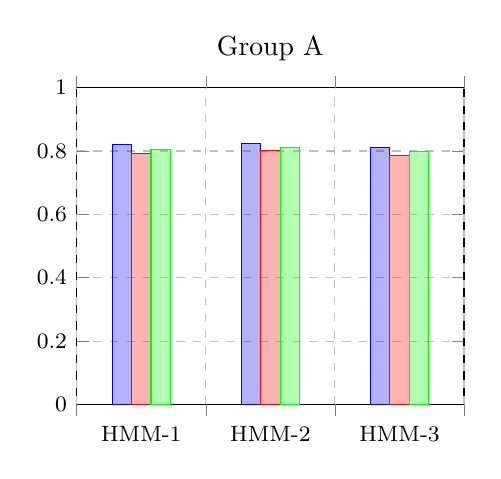
\begin{tikzpicture}
      \pgfplotsset{small}
      \begin{axis}[
        title={Group A},
        xmin=0.5, xmax=3.5,
        ymin=0, ymax=1,
        xticklabels={HMM-1,HMM-2,HMM-3},
        xtick={1,...,3},
        ytick={0,0.2,...,1},
        ybar=0pt,
        bar width=7pt,
        xtick distance=1,
        xtick style={
            /pgfplots/major tick length=0pt,
        },
        extra x ticks={-0.5,0.5,...,5.5},
        extra x tick labels=\empty,
        extra x tick style={
            grid=major,
            xtick style={
                /pgfplots/major tick length=4pt,
            },
        },
        ymajorgrids=true,
        grid style=dashed,
      ]

      \addplot[ybar, color=blue, fill=blue, fill opacity=0.3,] coordinates {
        (1,0.819)(2,0.823)(3,0.812)
      };
      \addplot[ybar, color=red, fill=red, fill opacity=0.3,] coordinates {
        (1,0.792)(2,0.802)(3,0.785)
      };
      \addplot[ybar, color=green, fill=green, fill opacity=0.3,] coordinates {
        (1,0.805)(2,0.812)(3,0.798)
      };
      \legend{};
       
      \end{axis}
    \end{tikzpicture}
    ~
    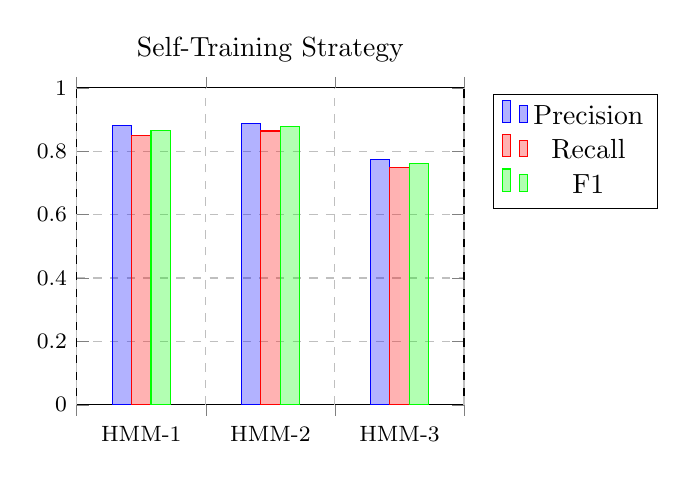
\begin{tikzpicture}
      \pgfplotsset{small}
      \begin{axis}[
        title={Self-Training Strategy},
        xmin=0.5, xmax=3.5,
        ymin=0, ymax=1,
        xticklabels={HMM-1,HMM-2,HMM-3},
        xtick={1,...,3},
        ytick={0,0.2,...,1},
        ybar=0pt,
        bar width=7pt,
        xtick distance=1,
        xtick style={
            /pgfplots/major tick length=0pt,
        },
        extra x ticks={-0.5,0.5,...,5.5},
        extra x tick labels=\empty,
        extra x tick style={
            grid=major,
            xtick style={
                /pgfplots/major tick length=4pt,
            },
        },
        ymajorgrids=true,
        grid style=dashed,
        % legend pos=north east,
	legend style={at={(1.5,0.8)},anchor=east},
      ]

      \addplot[ybar, color=blue, fill=blue, fill opacity=0.3,] coordinates {
        (1,0.880)(2,0.888)(3,0.774)
      };
      \addplot[ybar, color=red, fill=red, fill opacity=0.3,] coordinates {
        (1,0.850)(2,0.864)(3,0.750)
      };
      \addplot[ybar, color=green, fill=green, fill opacity=0.3,] coordinates {
        (1,0.865)(2,0.879)(3,0.762)
      };
      \legend{Precision, Recall, F1};
       
      \end{axis}
    \end{tikzpicture}

    \caption{Hidden Markov Models trained with the features in Group A and Group B.}
    \label{fig:hmm_self_training}
  \end{center}
\end{figure}

The self-trained models show a marked improvement in comparison
to the models with no self-training at the test set except for the third order \textit{HMM}.
With this, we conclude that the best \textit{HMM} for the name extraction task is a 
second-order \textit{HMM} using \textit{Group A} features and the self-training strategy. This
model achieves an \textit{F1} of 0.879. The detailed results for all HMMs is presented in
Table~\ref{tab:hmm_results}.


\begin{table}[h]
  \small
  \begin{center}
    \begin{tabular}{ lllllll }
      \toprule
      \multirow{2}{*}{Model} & \multicolumn{3}{c}{Validation} & \multicolumn{3}{c}{Test} \\
                             & \multicolumn{1}{c}{P} & \multicolumn{1}{c}{R} & \multicolumn{1}{c}{F1}
                             & \multicolumn{1}{c}{P} & \multicolumn{1}{c}{R} & \multicolumn{1}{c}{F1} \\
      \midrule
      \midrule
      HMM-1                           & 0.693 & 0.581 & 0.632 & 0.637 & 0.458 & 0.533 \\
      HMM-2                           & 0.703 & 0.630 & 0.665 & 0.653 & 0.527 & 0.583 \\
      HMM-3                           & 0.616 & 0.618 & 0.617 & 0.551 & 0.468 & 0.506 \\
      HMM-1 (Group A)                 & 0.813 & 0.816 & 0.814 & 0.819 & 0.792 & 0.805 \\
      HMM-2 (Group A)                 & 0.787 & 0.820 & 0.803 & 0.823 & 0.802 & 0.812 \\
      HMM-3 (Group A)                 & 0.774 & 0.816 & 0.795 & 0.812 & 0.785 & 0.798 \\
      HMM-1 (Group B)                 & 0.730 & 0.714 & 0.722 & 0.826 & 0.684 & 0.748 \\
      HMM-2 (Group B)                 & 0.720 & 0.710 & 0.715 & 0.820 & 0.724 & 0.769 \\
      HMM-3 (Group B)                 & 0.721 & 0.702 & 0.711 & 0.791 & 0.667 & 0.724 \\
      HMM-1 (Group A) + Self-Training & 0.752 & 0.876 & 0.810 & 0.880 & 0.851 & 0.865 \\
      HMM-2 (Group A) + Self-Training & 0.784 & 0.892 & 0.835 & \textbf{0.888} & 0.864 & \textbf{0.879} \\
      HMM-3 (Group A) + Self-Training & 0.789 & 0.891 & 0.837 & 0.774 & 0.750 & 0.762 \\
      HMM-1 (Group B) + Self-Training & 0.747 & 0.906 & 0.819 & 0.866 & 0.867 & 0.866 \\
      HMM-2 (Group B) + Self-Training & 0.771 & 0.912 & 0.835 & 0.885 & \textbf{0.869} & 0.877 \\
      HMM-3 (Group B) + Self-Training & 0.788 & 0.917 & 0.847 & 0.826 & 0.803 & 0.814 \\
      \bottomrule
    \end{tabular}
  \end{center}
  \caption{All \textit{Hidden Markov Models}}
  \label{tab:hmm_results}
\end{table}


\section{Conditional Random Fields}
\label{sec:experiments_crf}

When we compared a featureless Logistic Classifier with a featureless Naive Bayes model
we found that the Logistic Classifier performed significantly better. In this section we
want to check if CRFs are also better than HMMs when they use no features besides the
current word. Also, Linear Chain CRFs provide a much more flexible way to incorporate 
features in comparison to HMMs. When considering the application
of this class of models to the Researcher Name Extraction task, we want to understand how the feature
selection impacts the performance of the model.

\subsection{No Features}

Figure~\ref{fig:crf_no_features} shows a comparison between the Logistic Classifier
(that assumes label independence), the best Hidden Markov Model without features
and a CRF without features in the name extraction task. Different from the HMMs the 
discriminative models presented here resort to numerical optimization methods, therefore 
their parameters may vary between different runs, so we present the average result 
for each measure over five runs. In other sections, numerically optimized models will
follow the same rule.

\begin{figure}[h!]
  \begin{center}
    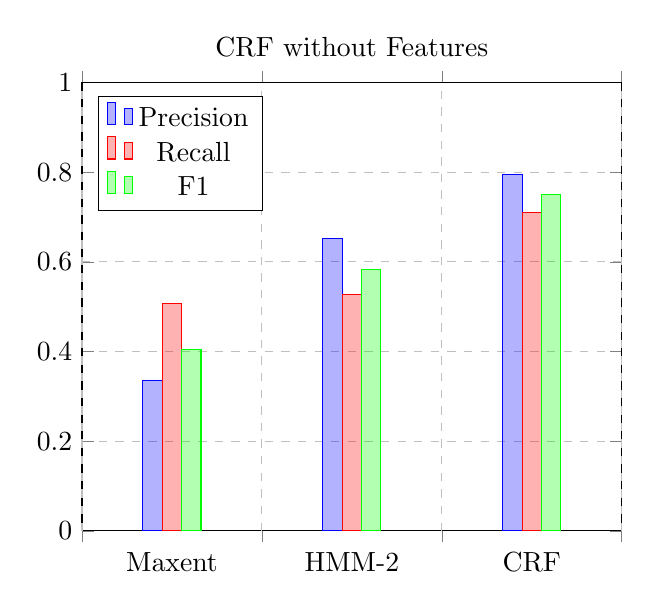
\begin{tikzpicture}
      \begin{axis}[
        title={CRF without Features},
        xmin=0.5, xmax=3.5,
        ymin=0, ymax=1,
        xticklabels={Maxent,HMM-2,CRF},
        xtick={1,...,3},
        ytick={0,0.2,...,1},
        ybar=0pt,
        bar width=7pt,
        xtick distance=1,
        xtick style={
            /pgfplots/major tick length=0pt,
        },
        extra x ticks={-0.5,0.5,...,5.5},
        extra x tick labels=\empty,
        extra x tick style={
            grid=major,
            xtick style={
                /pgfplots/major tick length=4pt,
            },
        },
        ymajorgrids=true,
        grid style=dashed,
        legend pos=north west,
      ]

      \addplot[ybar, color=blue, fill=blue, fill opacity=0.3,] coordinates {
        (1,0.335)(2,0.653)(3,0.795)
      };
      \addplot[ybar, color=red, fill=red, fill opacity=0.3,] coordinates {
        (1,0.508)(2,0.527)(3,0.710)
      };
      \addplot[ybar, color=green, fill=green, fill opacity=0.3,] coordinates {
        (1,0.404)(2,0.583)(3,0.750)
      };
      \legend{Precision, Recall, F1};
       
      \end{axis}
    \end{tikzpicture}
    \caption{
      Performance of the Maximum Entropy classifier, second-order Hidden Markov Models and 
      Linear Chain CRFs without features besides the current word on the test set of the NER on HTML dataset.
    }
    \label{fig:crf_no_features}
  \end{center}
\end{figure}

The \textit{CRF} model shows a significant improvement in comparison to the other models that used no features,
achieving an F1-score of 0.750. Next, we proceed to understand if the addition of features can improve this
performance further.


\subsection{Feature Selection}

To allow comparison between the \textit{HMMs} from the last section we consider \textit{CRFs} using features
from \textit{Group A} and \textit{Group B}. Figure~\ref{fig:crf_all_features} shows a comparison between 
the best \textit{HMM} for each group of features and the respective \textit{CRF} using the same group of features.

\begin{figure}[h!]
  \begin{center}
    \tiny
    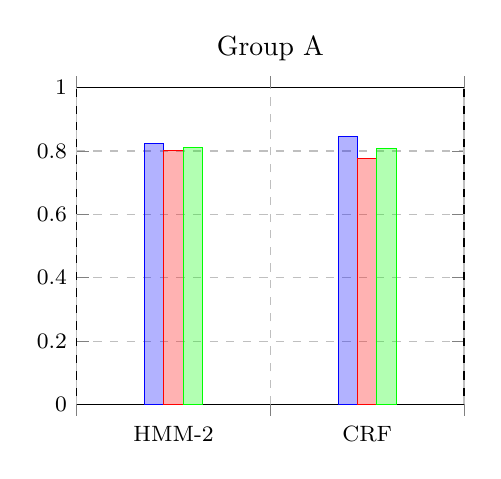
\begin{tikzpicture}
      \pgfplotsset{small}
      \begin{axis}[
        title={Group A},
        xmin=0.5, xmax=2.5,
        ymin=0, ymax=1,
        xticklabels={HMM-2,CRF},
        xtick={1,...,2},
        ytick={0,0.2,...,1},
        ybar=0pt,
        bar width=7pt,
        xtick distance=1,
        xtick style={
            /pgfplots/major tick length=0pt,
        },
        extra x ticks={-0.5,0.5,...,5.5},
        extra x tick labels=\empty,
        extra x tick style={
            grid=major,
            xtick style={
                /pgfplots/major tick length=4pt,
            },
        },
        ymajorgrids=true,
        grid style=dashed,
      ]

      \addplot[ybar, color=blue, fill=blue, fill opacity=0.3,] coordinates {
        (1,0.823)(2,0.845)
      };
      \addplot[ybar, color=red, fill=red, fill opacity=0.3,] coordinates {
        (1,0.802)(2,0.775)
      };
      \addplot[ybar, color=green, fill=green, fill opacity=0.3,] coordinates {
        (1,0.812)(2,0.808)
      };
      \legend{};
       
      \end{axis}
    \end{tikzpicture}
    ~
    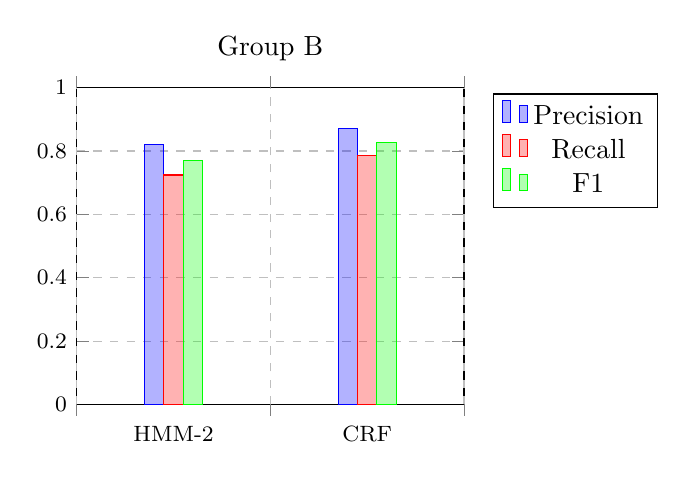
\begin{tikzpicture}
      \pgfplotsset{small}
      \begin{axis}[
        title={Group B},
        xmin=0.5, xmax=2.5,
        ymin=0, ymax=1,
        xticklabels={HMM-2,CRF},
        xtick={1,...,2},
        ytick={0,0.2,...,1},
        ybar=0pt,
        bar width=7pt,
        xtick distance=1,
        xtick style={
            /pgfplots/major tick length=0pt,
        },
        extra x ticks={-0.5,0.5,...,5.5},
        extra x tick labels=\empty,
        extra x tick style={
            grid=major,
            xtick style={
                /pgfplots/major tick length=4pt,
            },
        },
        ymajorgrids=true,
        grid style=dashed,
        % legend pos=north east,
	legend style={at={(1.5,0.8)},anchor=east},
      ]

      \addplot[ybar, color=blue, fill=blue, fill opacity=0.3,] coordinates {
        (1,0.820)(2,0.870)
      };
      \addplot[ybar, color=red, fill=red, fill opacity=0.3,] coordinates {
        (1,0.724)(2,0.786)
      };
      \addplot[ybar, color=green, fill=green, fill opacity=0.3,] coordinates {
        (1,0.769)(2,0.826)
      };
      \legend{Precision, Recall, F1};
       
      \end{axis}
    \end{tikzpicture}

    \caption{Linear Chain Conditional Random Fields trained with the features in Group A and Group B.}
    \label{fig:crf_all_features}
  \end{center}
\end{figure}

The CRF is more robust to variations in the feature selection. It performs
similar to the second-order HMM in Group A and slightly better in Group B, though
it tends towards an increase in precision rather than recall. The CRF is marginally better than
the HMM, however, when we consider the self-trained HMM-2, it still shows a better overall 
performance. 

There are two things that could still be tried to improve the CRF performance. First,
the CRF allows for a more flexible feature selection, so we could try adding more features,
since the correlation is not impeditive in this case. Second, we could try developing a self-training 
strategy for CRFs similar to the one employed on HMMs. However, Neural Networks 
showed a superior performance in many NLP tasks, so next, we consider neural architectures.
Table~\ref{tab:crf_results} presents the detailed results for CRFs at the name extraction
task in the validation and test sets.

\begin{table}[h]
  \small
  \begin{center}
    \begin{tabular}{ lllllll }
      \toprule
      \multirow{2}{*}{Model} & \multicolumn{3}{c}{Validation} & \multicolumn{3}{c}{Test} \\
                             & \multicolumn{1}{c}{P} & \multicolumn{1}{c}{R} & \multicolumn{1}{c}{F1}
                             & \multicolumn{1}{c}{P} & \multicolumn{1}{c}{R} & \multicolumn{1}{c}{F1} \\
      \midrule
      \midrule
      CRF                    & 0.806 & 0.805 & 0.806 & 0.795 & 0.710 & 0.750 \\
      CRF (Group A)          & 0.857 & 0.875 & 0.866 & 0.845 & 0.775 & 0.808 \\
      CRF (Group B)          & 0.881 & 0.903 & 0.892 & \textbf{0.870} & \textbf{0.786} & \textbf{0.826} \\
      \bottomrule
    \end{tabular}
  \end{center}
  \caption{All Conditional Random Fields.}
  \label{tab:crf_results}
\end{table}


\section{Neural Networks}
\label{sec:experiments_nn}

There are multiple Neural Network architectures that are suitable for solving 
\textit{Sequence Labeling} tasks. A model that has recently had remarkable success at 
solving these types of tasks is the BI-LSTM-CRF discussed in Section~\ref{sec:lstm_crf},
so we start our investigation by determining if it is also suited for the researcher
name extraction task. Additionaly, we want to determine if the CNN-based or LSTM-based
character representations can help improving the LSTM-CRF performance. We also want to
test if the Hard-Attention and Soft-Attention mechanisms for incorporating HTML structural
features provides any improvement. Finally, we want to understand if the F-score optimization
function can help controlling how much the model values precision in detriment of recall and
vice versa.


\subsection{Bi-LSTM-CRF with Glove-300 Embeddings}

One of the advantages of deep neural
networks is the fact that they can usually work without any feature engineering. 
Figure~\ref{fig:bi_lstm_crf} compares the performance of a \textit{BI-LSTM-CRF} on the test
set of the researcher name extraction task with the best \textit{HMM} and \textit{CRF} 
without features.

\begin{figure}[h!]
  \begin{center}
    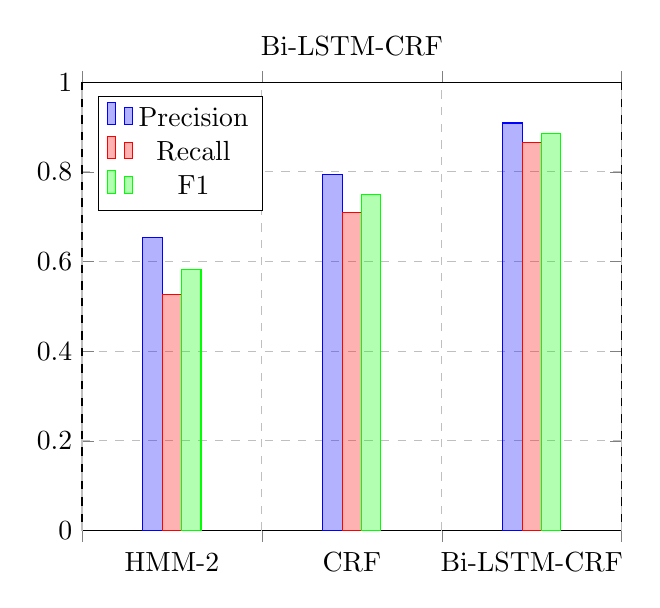
\begin{tikzpicture}
      \begin{axis}[
        title={Bi-LSTM-CRF},
        xmin=0.5, xmax=3.5,
        ymin=0, ymax=1,
        xticklabels={HMM-2,CRF,Bi-LSTM-CRF},
        xtick={1,...,3},
        ytick={0,0.2,...,1},
        ybar=0pt,
        bar width=7pt,
        xtick distance=1,
        xtick style={
            /pgfplots/major tick length=0pt,
        },
        extra x ticks={-0.5,0.5,...,5.5},
        extra x tick labels=\empty,
        extra x tick style={
            grid=major,
            xtick style={
                /pgfplots/major tick length=4pt,
            },
        },
        ymajorgrids=true,
        grid style=dashed,
        legend pos=north west,
      ]

      \addplot[ybar, color=blue, fill=blue, fill opacity=0.3,] coordinates {
        (1,0.653)(2,0.795)(3,0.909)
      };
      \addplot[ybar, color=red, fill=red, fill opacity=0.3,] coordinates {
        (1,0.527)(2,0.710)(3,0.865)
      };
      \addplot[ybar, color=green, fill=green, fill opacity=0.3,] coordinates {
        (1,0.583)(2,0.750)(3,0.886)
      };
      \legend{Precision, Recall, F1};
       
      \end{axis}
    \end{tikzpicture}
    \caption{
      Performance of the Bi-LSTM-CRF in comparison with the second-order Hidden Markov Models and 
      Linear Chain CRFs without features.
    }
    \label{fig:hmm_no_features}
  \end{center}
\end{figure}

The Bi-LSTM-CRF improves the performance of earlier models by a significant margin, though the
comparison is not completely fair, since we fed the model with Glove-300 word embeddings. However,
these pretrained embeddings are general to any language related task, so their incorporation in
does not require a lot of additional effort. Without any feature engineering, the Bi-LSTM-CRF model
already achieves an F1-score of 0.886, surpassing the best model up to this point (the HMM-2 with
self-training, which achieved 0.879 F1-score).


\subsection{Character Representations}
\label{ssec:char_representations}

Morphological features can help identifying named entities. We presented in Section~\ref{sec:char_representations}
two methods for incorporating character representations in \textit{Recurrent Neural Networks}, the \textit{CNN-based}
method, and the \textit{LSTM-based} method. In Table~\ref{tab:char_reps}, we compare the performance of
\textit{CNN} and \textit{LSTM} representations with the plain \textit{Bi-LSTM-CRF}.

\begin{table}[h]
  \small
  \begin{center}
    \begin{tabular}{ lllllll }
      \toprule
      Model & Precision & Recall & F1 \\
      \midrule
      Bi-LSTM-CRF                        & 0.909 (0.008) & 0.865 (0.020) & 0.886 (0.011) \\
      Bi-LSTM-CRF + CNN chars            & 0.921 (0.006) & 0.881 (0.005) & 0.901 (0.002) \\
      Bi-LSTM-CRF + LSTM chars           & 0.920 (0.007) & 0.886 (0.031) & 0.902 (0.019) \\
      Bi-LSTM-CRF (Group B)              & 0.921 (0.008) & 0.883 (0.022) & 0.901 (0.008) \\
      Bi-LSTM-CRF (Group B) + CNN chars  & 0.922 (0.006) & 0.868 (0.033) & 0.894 (0.018) \\
      Bi-LSTM-CRF (Group B) + LSTM chars & 0.913 (0.005) & 0.855 (0.021) & 0.883 (0.012) \\
      \bottomrule
    \end{tabular}
  \end{center}
  \caption{Bi-LSTM-CRF with Character Representations}
  \label{tab:char_reps}
\end{table}

The character representations improved the \textit{F1-score} by ~1.3 points. Also, both the 
\textit{CNN-based} and the \textit{LSTM-based} representations have a similar performance, yet 
the \textit{LSTM-based} representations are slightly better, owing probably to the fact that they 
can represent prefixes and suffixes while the \textit{CNN-based} filters are position 
invariant. 

We also present the results for these models using the features from \textit{Group B}. The
addition of features improves the performance of the plain \textit{Bi-LSTM-CRF}, but hurts the 
performance of the models with character representations.


\subsection{Attention Mechanisms}

The \textit{Self-Training} strategy for \textit{HMMs} showed that there is a lot to gain
from incorporating features related to the HTML structure in our models. The hard and soft
attention mechanisms proposed in Section~\ref{sec:attention} are two ways to do that. We 
compare the performance of the \textit{Bi-LSTM-CRF} with \textit{LSTM-based} character 
representations with the same model using a Hard Attention layer and a Soft Attention 
layer in Table~\ref{tab:attention}.

\begin{table}[h]
  \small
  \begin{center}
    \begin{tabular}{ lllllll }
      \toprule
      Model & Precision & Recall & F1 \\
      \midrule
      Bi-LSTM-CRF + LSTM chars           & 0.920 (0.007) & 0.886 (0.031) & 0.902 (0.019) \\
      ... + Hard Attention               & 0.925 (0.007) & 0.890 (0.011) & 0.907 (0.005) \\
      ... + Soft Attention               & 0.884 (0.025) & 0.849 (0.021) & 0.866 (0.013) \\
      \bottomrule
    \end{tabular}
  \end{center}
  \caption{Hard and Soft Attention}
  \label{tab:attention}
\end{table}

The \textit{Hard Attention} layer improved the original model by roughly 0.5 F1-score with the
bonus of reducing variance significantly. However,
the \textit{Soft Attention} actually hurt the performance significantly, what demands further 
explanation. The reason for this is probably that the \textit{Hard Attention} only captures if
the HTML context between two tags is exactly the same, but it does not look at what is this 
context. What the \textit{Hard Attention} layer learns is essentialy how much it can trust 
predictions made for words in the same HTML context, no matter what this context is. The 
\textit{Soft Attention} layer, however, also learns features about the HTML context, so
it can learn for example to look more at words that happen inside a <div> tag. This would not 
be problematic if all documents came from the same website, however, since this is not the case,
we cannot trust specific HTML configurations to be meaningful outside the document where they
happen. This does not mean that the \textit{Soft Attention} layer is useless, but for it to grasp
abstract structural patterns that could be useful, we would probably need a much larger dataset.


\subsection{Word Embeddings}

Up to this point, all neural architectures used Glove-300 pretrained word embeddings. However, the
choice of embeddings is of great importance to the success of neural sequence models. In fact, most
recent developments to the \textit{Named Entity Recognition} models come from the incorporation of 
better word embeddings rather than from different neural architectures. We considered three sets of
pretrained word embeddings in our experiments: Glove-300, Word2Vec-300 and Elmo.

Different from Glove-300 and Word2Vec-300, which are static, Elmo embeddings are context dependent and
need to be calculated for the specific dataset. This adds significant overhead to the model training.

Table~\ref{tab:word_embeddings} compares the performance of different sets of word embeddings in the
\textit{Bi-LSTM-CRF} model with \textit{LSTM-based} character representations.

\begin{table}[h]
  \small
  \begin{center}
    \begin{tabular}{ lllllll }
      \toprule
      Model & Precision & Recall & F1 \\
      \midrule
      Bi-LSTM-CRF + LSTM chars + Glove    & 0.920 (0.007) & 0.886 (0.031) & 0.902 (0.019) \\
      Bi-LSTM-CRF + LSTM chars + Word2Vec & 0.899 (0.011) & 0.831 (0.028) & 0.864 (0.019) \\
      Bi-LSTM-CRF + LSTM chars + Elmo     & 0.720 (0.033) & 0.885 (0.062) & 0.794 (0.043) \\
      \bottomrule
    \end{tabular}
  \end{center}
  \caption{Word Embeddings}
  \label{tab:attention}
\end{table}

As the results in Conll-2003 show, Glove-300 embeddings are superior to Word2Vec at the \textit{Named Entity Recognition}
task. However the \textit{ELMO} embeddings showed a very poor performance, contrasting to the great improvements
it showed in many NLP tasks, including NER. This is probably due to the fact that the pretrained \textit{Language Model} 
that generates the \textit{ELMO} embeddings has been trained on plain text, which is too different from the type of HTML
that we are dealing with.


\subsection{F-score Maximization}

Numerical optimization methods such as \textit{SGD} for training \textit{Deep Neural Networks} 
usually want to minimize the \textit{Cross Entropy}. However, what we ultimately care about
are the \textit{Precision} and \textit{Recall} measures. By reducing the \textit{Cross Entropy}, we
expect to increase these measures. But in Section~\ref{sec:fscore_optimization} we proposed to use
the \textit{F-score} expected utility function as an optimization objective for \textit{Deep Neural Networks}
on \textit{Sequence Labeling} tasks. We want to understand if, by using the optimization objective, we
can control how much the model prioritizes one measure over the other. Also, the results presented
in the last Section show that \textit{Neural Architectures} tend to value \textit{Precision} over
\textit{Recall} in the name extraction task, however it is arguably better to improve \textit{Recall} 
and lose a little bit of precision in this task, since it easier to filter out false positives from the
results than to find manually the false negatives in the corpus. Figure~\ref{fig:fscore_optimization}
presents the results on the test set for a \textit{Bi-LSTM-CRF} model with LSTM character representations
trained with the \textit{F-score} expected utility maximization objective and varying the objective
\textit{F-score} $ \alpha $. For example, $ \alpha=0.5 $ means that we value Recall as much as Precision,
$ \alpha=0.2 $ means that we value Precision twice as much as Recall, and $ \alpha=0.8 $ means that we value 
Recall twice as much as Precision.

\begin{figure}[h!]
  \begin{center}
    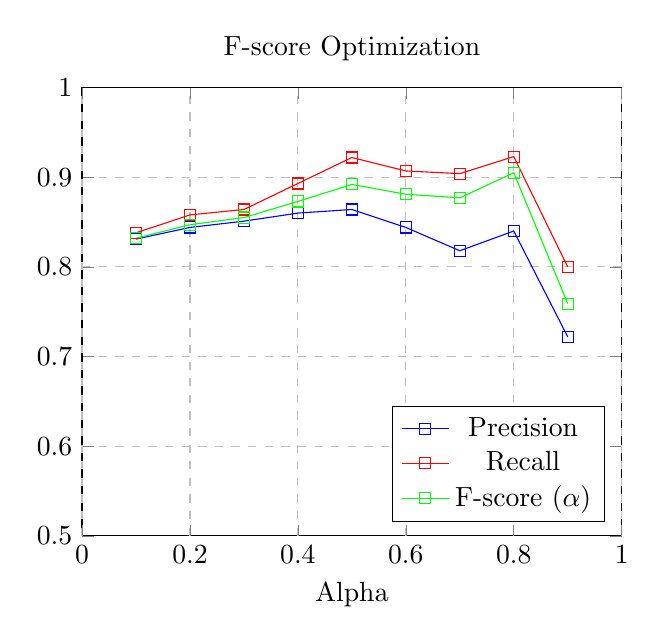
\begin{tikzpicture}
      \begin{axis}[
        title={F-score Optimization},
        xmin=0.0, xmax=1.0,
        ymin=0.5, ymax=1,
        xtick={0.0,0.2,...,1.0},
        ytick={0.5,0.6,...,1},
        xtick distance=1,
        xtick style={
            /pgfplots/major tick length=0pt,
        },
        xlabel={Alpha},
        extra x ticks={0.0,0.2,...,5.5},
        extra x tick labels=\empty,
        extra x tick style={
            grid=major,
            xtick style={
                /pgfplots/major tick length=4pt,
            },
        },
        ymajorgrids=true,
        grid style=dashed,
        legend pos=south east,
      ]


      \addplot[color=blue, color=blue,mark=square] coordinates {
        (0.1,0.831)(0.2,0.844)(0.3,0.851)(0.4,0.860)(0.5,0.864)(0.6,0.844)(0.7,0.818)(0.8,0.840)(0.9,0.722)
      };
      \addplot[color=red, color=red,mark=square] coordinates {
        (0.1,0.838)(0.2,0.858)(0.3,0.864)(0.4,0.893)(0.5,0.922)(0.6,0.907)(0.7,0.904)(0.8,0.923)(0.9,0.800)
      };
      \addplot[color=green, color=green,mark=square] coordinates {
	(0.1,0.832)(0.2,0.847)(0.3,0.855)(0.4,0.873)(0.5,0.892)(0.6,0.881)(0.7,0.877)(0.8,0.905)(0.9,0.759)
      };
      \legend{Precision, Recall, F-score ($ \alpha $)};
       
      \end{axis}
    \end{tikzpicture}
    \caption{
      Precision, Recall and F-scores as we vary $ \alpha $ for the Bi-LSTM-CRF with LSTM character 
      representations optimizing the expected F-score function directly 
    }
    \label{fig:fscore_loss}
  \end{center}
\end{figure}

The experiment shows that the capacity to control how much the model optimizes for one measure over the
other is very limited. Even when giving a lot more priority to Precision ($ \alpha=0.1 $), the model is still
less precise than the variant that optimizes for the F1-score ($ \alpha=0.5 $). Actually, the model that achieves
top Precision (0.864) and the second best Recall (0.922) is the one with $ \alpha=0.5 $. The model with 
$ \alpha=0.8 $ achieves the best Recall (0.923).

An interesting result that we can observe in the models that optimized the expected F-score function is that
all of them valued \textit{Recall} over \textit{Precision}. A result that contrasts with the 
\textit{Neural Networks} that were presented earlier, which prioritized \textit{Precision}. Table~\ref{tab:fscore_optimization}
shows the detailed results from the models discussed in this Section.

\begin{table}[h]
  \small
  \begin{center}
    \begin{tabular}{ lllllll }
      \toprule
      Alpha & Precision & Recall & F-score ($ \alpha $) \\
      \midrule
       % 0.1 & 0.879 (0.007) & 0.925 (0.012) & 0.884 (0.006) & 0.831 (0.010) & 0.838 (0.014) & 0.832 (0.009) \\ 
       % 0.2 & 0.876 (0.001) & 0.939 (0.003) & 0.888 (0.000) & 0.844 (0.009) & 0.858 (0.013) & 0.847 (0.010) \\
       % 0.3 & 0.881 (0.005) & 0.935 (0.007) & 0.896 (0.004) & 0.851 (0.011) & 0.864 (0.014) & 0.855 (0.011) \\
       % 0.4 & 0.873 (0.008) & 0.962 (0.010) & 0.907 (0.004) & 0.860 (0.010) & 0.893 (0.012) & 0.873 (0.007) \\
       % 0.5 & 0.823 (0.005) & 0.970 (0.008) & 0.890 (0.000) & 0.864 (0.037) & 0.922 (0.027) & 0.892 (0.032) \\
       % 0.6 & 0.839 (0.011) & 0.976 (0.003) & 0.916 (0.005) & 0.844 (0.004) & 0.907 (0.013) & 0.881 (0.010) \\
       % 0.7 & 0.810 (0.007) & 0.975 (0.003) & 0.919 (0.002) & 0.818 (0.018) & 0.904 (0.005) & 0.877 (0.009) \\
       % 0.8 & 0.814 (0.009) & 0.980 (0.002) & 0.942 (0.001) & 0.840 (0.006) & 0.923 (0.011) & 0.905 (0.010) \\
       % 0.9 & 0.680 (0.081) & 0.900 (0.055) & 0.871 (0.060) & 0.636 (0.085) & 0.752 (0.048) & 0.738 (0.053) \\
       0.1 & 0.831 (0.010) & 0.838 (0.014) & 0.832 (0.009) \\ 
       0.2 & 0.844 (0.009) & 0.858 (0.013) & 0.847 (0.010) \\
       0.3 & 0.851 (0.011) & 0.864 (0.014) & 0.855 (0.011) \\
       0.4 & 0.860 (0.010) & 0.893 (0.012) & 0.873 (0.007) \\
       0.5 & 0.864 (0.037) & 0.922 (0.027) & 0.892 (0.032) \\
       0.6 & 0.844 (0.004) & 0.907 (0.013) & 0.881 (0.010) \\
       0.7 & 0.818 (0.018) & 0.904 (0.005) & 0.877 (0.009) \\
       0.8 & 0.840 (0.006) & 0.923 (0.011) & 0.905 (0.010) \\
       0.9 & 0.636 (0.085) & 0.752 (0.048) & 0.738 (0.053) \\
      \bottomrule
    \end{tabular}
  \end{center}
  \caption{F-score optimization}
  \label{tab:fscore_optimization}
\end{table}


\subsection{Technical Details for Neural Networks}

All neural models were trained with the Adam Optimizer using a learning rate of 0.001 over 20 epochs on minibatches
of size 10. We used early stopping \cite{Caruana2000} to select the best 
parameters, considering the F1 measure in the validation set. All \textit{Bi-LSTM-CRF} models contained a 
single LSTM layer with 100 weights. Dropout layers with 0.5 dropout rates were added after the LSTM, 
the character representations, and the attention matrix when applicable. The neural models were trained on 
Amazon G3.4xlarge instances, which use NVIDIA Tesla M60 GPUs with 8GB internal memory. The implementations
were done entirely in Python using Google's Tensorflow deep learning library. 


\section{What model is best?}
\label{sec:experiments_best}

We have discussed multiple sequence labeling methods in the previous Sections and now we provide
an overview of the best variants of each category.
In Table~\ref{tab:best_models}, we compare the performance of the best \textit{HMMs}, 
\textit{CRFs} and \textit{Neural Networks} on the test set of the NER on HTML dataset.

\begin{table}[h]
  \small
  \begin{center}
    \begin{tabular}{ lllllll }
      \toprule
      Model & Precision & Recall & F1 \\
      \midrule
       % HMM-2 (No features)                        & 0.703 & 0.630 & 0.665 & 0.653 & 0.527 & 0.583 \\
       % HMM-2 (Group A)                            & 0.787 & 0.820 & 0.803 & 0.823 & 0.802 & 0.812 \\
       % HMM-2 (Group A) + Self-Training            & 0.784 & 0.892 & 0.835 & 0.888 & 0.864 & 0.879 \\
       % CRF (No features)                          & 0.806 & 0.805 & 0.806 & 0.795 & 0.710 & 0.750 \\
       % CRF (Group B)                              & 0.881 & 0.903 & 0.892 & 0.870 & 0.786 & 0.826 \\
       HMM-2 (Group A)                            & 0.823         & 0.802         & 0.812                  \\
       HMM-2 (Group A) + Self-Training            & 0.888         & 0.864         & 0.879                  \\
       CRF (Group B)                              & 0.870         & 0.786         & 0.826                  \\
       Bi-LSTM-CRF + LSTM chars                   & 0.920 (0.007) & 0.886 (0.031) & 0.902 (0.019)          \\
       Bi-LSTM-CRF + LSTM chars + Hard Attention  & 0.925 (0.007) & 0.890 (0.011) & \textbf{0.907 (0.005)} \\
       Bi-LSTM-CRF + LSTM chars + F1 Optimization & 0.864 (0.037) & 0.922 (0.027) & 0.892 (0.032)          \\
      \bottomrule
    \end{tabular}
  \end{center}
  \caption{Overview of the best models for the name extraction task in the NER on HTML dataset}
  \label{tab:best_models}
\end{table}

If we take the \textit{F1} score as the comparison criterium, then the \textit{Bi-LSTM-CRF} with LSTM 
character representations, Glove-300 embeddings, and a Hard Attention Layer is the winning model with an
\textit{F1} of 0.907. However, as we previously argued, \textit{Recall} should be privileged over 
\textit{Precision} in this task. When we take this in consideration, the \textit{Bi-LSTM-CRF} optimized
with the \textit{Expected F-score} objective is probably a better option, but its variance is significantly 
higher.

Despite the superior performance of \textit{Neural Networks} in this task, there remains an important 
consideration to be made. As we increase the complexity and training time required by our models, there 
is only a scant gain in terms of \textit{Precision} and \textit{Recall}. For example, lets compare the 
\textit{Bi-LSTM-CRF} with a Hard Attention Layer and the \textit{HMM-2} using Self-training strategy.
The first model achieved an 0.907 $ \pm 0.005 $ \textit{F1-score} in comparison to the 0.879 F1-score 
achieved by the latter. This is a 0.028 increase, which is not bad, but it comes to mind if the added
complexity is entirely justifiable. 

The \textit{Neural Network} approach does not demand any feature engineering or special
training strategy, contrasting with the \textit{HMM} approach, which is highly reliant on
the right selection of features and the self-training strategy. However, the absence of
human intervention on \textit{Neural Network} training is questionable since we need to
define a number of hyper parameters (e.g. learning rate, momentum, weight decay, etc.) and
many details about the neural architecture, such as the number of \textit{LSTM} layers and
hidden weights, where to add dropout layers, which word embeddings to use, etc. In summary, there
are many choices to be made, none of which have a definitive justification, and all of them
can impact model performance (especially the dropout layers and word embeddings). 

To the best of our abilities, the TensorFlow implementation of the Bi-LSTM-CRF + LSTM chars + 
Hard Attention model running on an AWS GPU instance took approximately 6075 seconds to train 
and run predictions in the test set. While, the \textit{HMM-2} did the same in approximately
64 seconds, running in a conventional CPU. That is almost a hundred times faster. Finally, if 
we consider the intellectual cost of understanding and implementing both models and the code 
maintainability of both implementations, the difference gets even more profound.

So, what model is best? It depends on the end goal. If the goal is to achieve as much accuracy
as possible, then definitely go for \textit{Deep Neural Architectures}. However, for most
ordinary implementations, simpler models should probably be preferred. In both cases, models
trained on publically available sequence tagging datasets will probably perform rather poorly,
so most of the effort would certainly be better spent on constructing task specific datasets
of high quality. This points to the necessity of searching for good unsupervised approaches to 
sequence labeling. This way, we would have models with better flexibility and good accuracy in
many extraction tasks. Unfortunately, unsupervised and semi supervised approaches to this problem 
are still far from serviceable.

\subsection{Heuristic Filtering}

Despite the variation between the sequence models presented above, they tend to commit some
similar prediction mistakes. We tried a simple heuristic strategy to test how difficult
it would be to filter out false positives from the results. We automatically relabeled tokens
that were labeled as a person ("B-PER" or "I-PER") to an outside ("O") label if:

\begin{itemize}
\item It was an honorific (Mr., Dr., P.hD., etc.).
\item It contained a number.
\item It was a punctuation sign just before or after a name (e.g. "- Mark" or "Emma ;").
\item It was an isolated name label.
\item It belonged to a name that was repeated at least three times.
\end{itemize}

The results of the heuristic filtering strategy for the best models is presented in 
Table~\ref{tab:heuristic_filtering}.

\begin{table}[h]
  \small
  \begin{center}
    \begin{tabular}{ lllllll }
      \toprule
      Model & Precision & Recall & F1 \\
      \midrule
       HMM-2 (Group A)                            & 0.9240 & 0.8795 & 0.9012 \\
       CRF (Group B)                              & 0.9236 & 0.7951 & 0.8545 \\
       Bi-LSTM-CRF + LSTM chars                   & 0.9387 & 0.8887 & 0.9130 \\
       Bi-LSTM-CRF + LSTM chars + Hard Attention  & 0.9376 & 0.8997 & 0.9183 \\
       Bi-LSTM-CRF + LSTM chars + F1 Optimization & 0.9239 & 0.9409 & 0.9323 \\
      \bottomrule
    \end{tabular}
  \end{center}
  \caption{Overview of the best models for the name extraction task in the NER on HTML dataset}
  \label{tab:heuristic_filtering}
\end{table}

The results for the \textit{Heuristic Filtering Strategy} show that the precision of all models could 
be improved considerably with a very simple approach. This implies that the number of false 
positives is not such a big problem on extraction tasks, since the mistakes commited by the classifiers
are at least to some extext quite repetitive.

\section{Summary}

Baochikawawau.


\chapter{Related Work}

\section{Web Information Extraction}

In the last 20 years, the astonishing growth of public information in the Web has 
led to the development of a number of different approaches to the problem of Web 
data extraction. Traditionally, the task was solved by designing special purpose
programs called wrappers to recognize relevant data and store records in a structured
format. These early tools varied wildly relative to their degree of automation. 

It was readily perceived that manual wrapper generation was a rather tedious and
error prone process, unsuited for large scale operations. Wrappers tend to
break frequently because they rely heavily on webpage features that can change 
often. So, in the late nineties, several authors advocated for wrapper induction, a technique 
that consists of automatically constructing wrappers from a small set of examples by 
identifying delimiters or context tokens that single out the desired attributes. 
Some remarkable wrapper induction methods are WIEN \cite{Kushmerick2000}, Soft 
Mealy \cite{Hsu1998} and STALKER \cite{Muslea1999}.

Despite being better than constructing wrappers manually, wrapper induction methods 
still suffered from a lack of expressive power and flexibility. These methods had 
trouble handling records with missing attributes or unusual structures because
patterns could only be identified if they happened at least once in the examples.

Other approaches such as NoDoSE \cite{Adelberg1998} and Debye \cite{Laender2002a} 
brought greater flexibility to wrapper induction methods by requiring a greater level 
of human interaction through graphical user interfaces. Web data extraction techniques often 
require some sort of assistance from human experts to boost accuracy. One of the main challenges 
in the field lies in determining an adequate trade-off between the degree of automation and 
the precision and recall of the data extraction tool.

To automate the task of Web data extraction completely some approaches,
such as Road Runner \cite{Crescenzi2001}, removed entirely the need for data examples.
Road Runner parses documents belonging to a same class (e.g. books on Amazon) and 
generates wrappers based on their similarities and differences, yielding comparable results 
to those obtained by wrapper induction methods. However, like previous approaches, it was 
unsuited for cross site extraction tasks because the learned rules were not general enough.

NLP based approaches aimed at extracting more general rules that could possibly
be employed over multiple websites. RAPIER \cite{Califf1999} is a method of rule
extraction that uses information such as part-of-speech tags and semantic classes from
a lexicon to derive patterns from a set of training examples. This approach is more
flexible than the wrapper induction methods, however it achieves much lower rates of 
recall and precision.

In 2002, a survey by Laender et al. \cite{Laender2002} made a thorough classification of the
early approaches with a taxonomy based on their main technology, being them: languages for
wrapper development, HTML-aware tools, NLP-based tools, Wrapper Induction Tools,
Modeling-based tools and Ontology-based tools. Some noteworthy examples from this era
are: 

\begin{itemize}
\item TSIMMIS \cite{Hammer1997} and WebOQL \cite{Arocena1999}, which are special purpose 
languages for building wrappers.

\item Road Runner \cite{Crescenzi2001}, XWRAP \cite{Liu2000} and W4F \cite{Sahuguet1999}, 
which are HTML-aware tools that infer meaningful patterns from the HTML structure.

\item RAPIER \cite{Califf1999}, SRV \cite{Freitag1998}, WHISK \cite{Soderland1999}, which 
are NLP-based tools.

\item WIEN \cite{Kushmerick2000}, Soft Mealy \cite{Hsu1998} and STALKER \cite{Muslea1999} which 
are wrapper induction methods.

\item NoDoSE \cite{Adelberg1998} and Debye \cite{Laender2002a}, which are semi supervised modeling
based tools that require some interaction with the user by means of a graphical
user interface.
\end{itemize}

In 2006, Chang et al. \cite{Chang2006} complemented the previous surveys with semi-supervised 
technologies such as Thresher \cite{Hogue2005}, IEPAD \cite{Chang2001} and 
OLERA \cite{Chang2004}. They differed from supervised 
and unsupervised methods because they either needed only a rough description of
data from users for extraction rule generation or some level of post processing
that needed user attention. The survey also mentioned newer unsupervised methods
such as DeLa \cite{Wang2003}, Exalg \cite{Arasu2003} and Depta \cite{Zhai2005}.

Most of the early information extraction systems were rule-based with either 
manual rule description or automatic rule learning from examples, thus they
suffered from a lack of flexibility when dealing with noisy and unstructured data.
Huge progress in the field of statistical learning led to the development of
models that tried to solve this problem.

In 2008, Sarawagi \cite{Sarawagi2008} introduced a classification that segmented wrappers in
rule-based methods, statistical methods and hybrid models, bringing together 
the fields of named entity recognition, relationship extraction and information extraction. 
The rule based methods encompass most of the previous models. While the statistical methods 
convert the extraction task into a token labeling task, solved with Named Entity Recognition 
and Relationship Extractions methods. Traditionally, these subtasks were solved with 
generative models based on Hidden Markov Models or discriminative models based on the 
Maximum Entropy principle, but recently these have been largely superseded by Deep Neural 
Networks. Different from automatic wrapper generators, statistical methods are suitable for
a large variety of tasks, especially when we want the system to handle cross website information 
extraction and plain text information extraction. That is why this class of methods is of 
special interest to our application. The progress of Statistical models will be 
discussed in the next Section.

Surveys by Ferrara et al. \cite{Ferrara2014}, Schulz et al. \cite{Schulz2016} and 
Varlamov et al. \cite{Varlamov2016} updated the previous surveys on information 
extraction methods with some interesting innovations. 
Some examples are: the Visual Box Model \cite{Krupl2005}, a data extraction system that produces 
a visualization of the webpage to exploit visual cues to identify records presented in a tabular form;
automatic wrapper adaptation \cite{Ferrara2011}, a technique that tries to reduce the cost of 
wrapper maintenance by measuring the similarity of HTML trees and adapting
wrappers to the new page structure; AutoRM \cite{Shi2015}, a method to mine
records from a single webpage by identifying similar data regions through DOM
tree analysis; Knowledge Vault \cite{Dong2014}, a method that combines different 
extraction approaches to feed a probabilistic knowledge base.

Most data extraction systems focus on extracting information from single websites
and are therefore unsuited for cross website extraction tasks. Even unsupervised
approaches that are domain independent, such as RoadRunner \cite{Crescenzi2001} 
and EXALG \cite{Arasu2003} only work well for extracting data from pages generated 
from a same template. 

A statistical approach to unsupervised domain 
independent Web data extraction was described by Zhu et al \cite{Zhu2005}. The 2D CRF 
model takes a webpage segmented into data blocks and employs a two dimensional conditional 
random field model to perform attribute labeling. The model was further improved
\cite{Zhu2006} to model record segmentation and attribute labeling as a joint task.
Some of the limitations of early unsupervised methods 
were also tackled by ObjectRunner \cite{Abdessalem2010} and AMBER \cite{Furche2012}. 
These methods work by annotating webpages automatically with regular expressions, gazetteers and 
knowledge bases. They can rectify low quality annotations and even improve the annotators
by exploring regular structures in the DOM during the record segmentation phase.

Web data extraction methods have undoubtedly improved extraordinarily, but
as pointed by Schulz et al. \cite{Schulz2016}, it is difficult to compare the results 
achieved by competing tools, and many seem to rely excessively on heuristic methods.
In that regard, the recent advancements in sequence taggers may provide more robust and
flexible extraction tools.

\section{Named Entity Recognition}

\textit{Named Entity Recognition} is an important subtask of \textit{Information Extraction},
together with \textit{Relationship Extraction} and \textit{Named Entity Linking}.
In the context of the researcher name extraction task, we are evaluating the 
performance of different systems only in this subtask.
As previously discussed in Chapter~\ref{cha:problem_discussion}, the 
\textit{Named Entity Recognition} task was introduced in the Third Message 
Understanding Conference (MUC-3) (CITE), where researchers were asked to extract
entities from a news corpus about terrorist incidents. But, it was the 
language-independent Named Entity Recognition shared task at the Conference 
on Computational Natural Language Learning in 2003 (CONLL-2003)~\cite{KimSang2003} 
that established an enduring labeled dataset constructed with news texts from Reuters.
Despite its reduced size and the limited variability of its documents, the CONLL-2003 
dataset is still used to compare the performance of different NER systems in English, and 
German. 

Sequence labeling for NER and part-of-speech tags (labeling nouns, verbs, pronouns, etc.) 
is very similar, so, many times, research articles report results for systems
on both tasks. And, frequently, the best methods for the former task are also the best 
methods for the latter task.

Traditionally, the NER task was solved with generative models based on 
\textit{Hidden Markov Models} (HMMs). The first appearances of HMMs in the
field of Natural Language Processing occurred in the mid-seventies and were
primarily focused on the problem of Speech Recognition. 
In the late nineties, HMMs also found important applications in Information 
Extraction and NER \cite{Leek1997, Bikel1999, Freitag1999, Freitag2000}.

% A. Borthwick, J. Sterling, E. Agichtein, and R. Grishman, "Exploiting diverse
% knowledge sources via maximum entropy in named entity recognition," in Sixth
% Workshop on Very Large Corpora New Brunswick, New Jersey, Association for
% Computational Linguistics, 1998.

% [Bikelrfa/. , 1999] D. Bikel, R. Schwartz, and R. Weischedel. 
% An algorithm that learns what's in a  name. Machine Learning, 34(1 ):211-231, 1999. 

% [Freitag and McCallum, 2000] D. Freitag and A. McCallum. Information extraction with HM M structures learned by stochastic optimization. 

The problem with HMMs was primarily that it modeled the joint probability between 
sequences of observations and labels $ P(X, Y) $, a harder problem than modelling the corresponding 
conditional probability $ P(Y|X) $. It assumed a prior distribution for the observations $ X $, and
therefore, it could not handle any selection of features. This lack of flexibility led to the 
development of discriminative approaches to sequence labeling.

Some early examples are Maximum Entropy Taggers for NER~\cite{Borthwick1998} and
POS-Tagging~\cite{Ratnaparkhi1998}. The Maximum Entropy Markov Model~\cite{McCallum2000} 
was developed just a while later, building up on the intuition of HMMs combined with
the flexibility of discriminative approaches. However, because of the label bias problem,
this model was superseded by Conditional Random Fields~\cite{Lafferty2001, McCallum2003} (CRF). 
% https://aclweb.org/anthology/W03-0425.
At this time, the best performing systems almost always resorted to external gazetteers 
and hand-chosen features~\ref{Florian2003}.

With the advancement of \textit{Machine Learning} in recent years, we saw the rise
of \textit{Neural Networks} for \textit{Sequence Labeling}. In 2011, \cite{Collobert2011} 
introduced Neural Networks free of feature engineering to \textit{Sequence Labeling},
using a Convolutional Neural Network over word embeddings with a CRF output layer to tackle 
the problems of POS-tagging, Chunking, Semantic Role Labeling, and NER. A similar architecture 
proposed in 2015 by~\cite{Huang2015}, the LSTM-CRF, replaced the CNN in \cite{Collobert2011} 
with a bidirectional LSTM, achieving better results.

In 2016, further advancement to the NER models was achieved by incorporating character 
representations at the bottom of the LSTM-CRF archictecture to extract morphological 
features from the words automatically. The model by~\cite{Lample2016} uses a 
bidirectional LSTM over character embeddings and the model by~\cite{Ma2016} uses a
one dimensional CNN with max pooling over character embeddings.

Small improvements to NER systems have been made since then, primarily due to the 
introduction of new Word Embeddings on variations of the LSTM-CRF architecture. From
this group, we can mention ElMO~\cite{Peters2018}, Bert~\cite{Devlin2018}, and
Flair~\cite{Akbik2018}. 
% https://arxiv.org/abs/1802.05365
% https://arxiv.org/abs/1810.04805
% https://drive.google.com/file/d/17yVpFA7MmXaQFTe-HDpZuqw9fJlmzg56/view
All of them were introduced in 2018, and they differ primarily 
in how to construct contextual embeddings from the internal states of a language model.
To our knowledge, the best NER system up to this date (considering the Conll-2003 dataset)
is the bidirectional transformer model proposed by~\cite{Baevksi2019} in 2019 that used
a stack of self attention modeules and Elmo embeddings. Table~\ref{tab:ner_model_comparison}
shows a comparison of the reported F1 scores for each one of the neural models
discussed in this Section and the model that won the challenge in 2003~\ref{Florian2003}.
Many models that held the best F1-score at one point or another were omitted from this
table.

\begin{table}[h]
  \small
  \begin{center}
    \begin{tabular}{ ll }
      \toprule
      Model & Test F1 \\
      \midrule
       Florian et al 2003 (CONLL-2003 Winner)      & 88.76 \\
       Collobert et al 2011                        & 89.59 \\
       Huang 2015                                  & 90.10 \\
       Lample 2016                                 & 90.94 \\
       Ma 2016                                     & 91.21 \\
       Elmo Peters 2018                            & 92.22 \\
       Bert Devlin 2018                            & 92.80 \\
       Flair Akbik 2018                            & 93.09 \\
       Baevski 2019                                & 93.50 \\
      \bottomrule
    \end{tabular}
  \end{center}
  \caption{}
  \label{tab:heuristic_filtering}
\end{table}

\chapter{Conclusion and Future Work}

Machine-learning-based sequence labeling models provide a flexible approach to Web data 
extraction, in contrast to more traditional methods. In simple cases, a neural
named entity tagger may be sufficient to solve the entire data extraction task. In 
other cases, the sequence tagger remains an important part of the web data extraction
system, as it performs attribute labeling on data records with accuracy and flexibility.

In this article, we compared the performance of different sequence models on the task of
named entity recognition on HTML, introducing a novel dataset that is publicly available. 
We found that there are two components to the most successful models: neural based character 
representations that extract morphological features automatically, and the joint modelling 
of output labels.

We showed that a BI-LSTM-CRF neural network with LSTM-based character representations can 
be employed effectively to solve a web data extraction task, achieving an F1-score of 
0.8867 with no feature engineering on the faculty listings dataset.

The effective recognition of named entities on HTML is an essential step in most general 
Web data extraction methods. The accuracy achieved by deep neural architectures even
on webpages that are very different from the plain text for which these architectures 
were initially designed shows the potential for a truly flexible approach to cross domain 
web data extraction.


\ppgccbibliography{bibfile}


% \begin{appendices}
% \label{app:html_segmenter}
% 
% \chapter{HTML sentence segmenter}
% 
% Lorem ipsum dolor.
% 
% \chapter{Outro ap�ndice}
% 
% \dummytxta
% 
% \end{appendices}
% 
% 
% \begin{attachments}
% 
% % Para cada anexo, um \chapter
% \chapter{Um anexo}
% 
% \dummytxta
% 
% \chapter{Outro anexo}
% 
% \dummytxta
% \end{attachments}


\end{document}
